%%%%%%%%%%%%%%%%%%%%%%%%%%%%%%%%%%%%%%%%%
% Beamer Presentation
% LaTeX Template
% Version 1.0 (10/11/12)
%
% This template has been downloaded from:
% http://www.LaTeXTemplates.com
%
% License:
% CC BY-NC-SA 3.0 (http://creativecommons.org/licenses/by-nc-sa/3.0/)
%
%%%%%%%%%%%%%%%%%%%%%%%%%%%%%%%%%%%%%%%%%

%----------------------------------------------------------------------------------------
%    PACKAGES AND THEMES
%----------------------------------------------------------------------------------------

\documentclass[usenames,dvipsnames]{beamer}
\usepackage{animate}
\usepackage{float}
\usepackage{bm}
\usepackage{mathtools}
\usepackage{extarrows}
\usepackage[utf8]{inputenc}
\usepackage[english]{babel}
\usepackage{minted}
\newcommand{\ChoL}{\mathsf{L}}
\newcommand{\bx}{\mathbf{x}}
\newcommand{\ii}{\mathrm{i}}
\newcommand{\bxi}{\bm{\xi}}
\newcommand{\bmu}{\bm{\mu}}
\newcommand{\bb}{\mathbf{b}}
\newcommand{\bA}{\mathbf{A}}
\newcommand{\bJ}{\mathbf{J}}
\newcommand{\bB}{\mathbf{B}}
\newcommand{\bM}{\mathbf{M}}

\newcommand{\by}{\mathbf{y}}
\newcommand{\bw}{\mathbf{w}}

\newcommand{\bX}{\mathbf{X}}
\newcommand{\bY}{\mathbf{Y}}
\newcommand{\bs}{\mathbf{s}}
\newcommand{\sign}{\mathrm{sign}}
\newcommand{\bt}[0]{\bm{\theta}}
\newcommand{\bc}{\mathbf{c}}
\newcommand{\bzero}{\mathbf{0}}
\renewcommand{\bf}{\mathbf{f}}
\newcommand{\bu}{\mathbf{u}}
\newcommand{\bv}[0]{\mathbf{v}}

\mode<presentation> {

% The Beamer class comes with a number of default slide themes
% which change the colors and layouts of slides. Below this is a list
% of all the themes, uncomment each in turn to see what they look like.

%\usetheme{default}
%\usetheme{AnnArbor}
%\usetheme{Antibes}
%\usetheme{Bergen}
%\usetheme{Berkeley}
%\usetheme{Berlin}
%\usetheme{Boadilla}
%\usetheme{CambridgeUS}
%\usetheme{Copenhagen}
%\usetheme{Darmstadt}
%\usetheme{Dresden}
%\usetheme{Frankfurt}
%\usetheme{Goettingen}
%\usetheme{Hannover}
%\usetheme{Ilmenau}
%\usetheme{JuanLesPins}
%\usetheme{Luebeck}
\usetheme{Madrid}
%\usetheme{Malmoe}
%\usetheme{Marburg}
%\usetheme{Montpellier}
%\usetheme{PaloAlto}
%\usetheme{Pittsburgh}
%\usetheme{Rochester}
%\usetheme{Singapore}
%\usetheme{Szeged}
%\usetheme{Warsaw}


% As well as themes, the Beamer class has a number of color themes
% for any slide theme. Uncomment each of these in turn to see how it
% changes the colors of your current slide theme.

%\usecolortheme{albatross}
\usecolortheme{beaver}
%\usecolortheme{beetle}
%\usecolortheme{crane}
%\usecolortheme{dolphin}
%\usecolortheme{dove}
%\usecolortheme{fly}
%\usecolortheme{lily}
%\usecolortheme{orchid}
%\usecolortheme{rose}
%\usecolortheme{seagull}
%\usecolortheme{seahorse}
%\usecolortheme{whale}
%\usecolortheme{wolverine}

%\setbeamertemplate{footline} % To remove the footer line in all slides uncomment this line
%\setbeamertemplate{footline}[page number] % To replace the footer line in all slides with a simple slide count uncomment this line

%\setbeamertemplate{navigation symbols}{} % To remove the navigation symbols from the bottom of all slides uncomment this line
}
\usepackage{booktabs}
\usepackage{makecell}
\usepackage{soul}
\newcommand{\red}[1]{\textcolor{red}{#1}}
%
%\usepackage{graphicx} % Allows including images
%\usepackage{booktabs} % Allows the use of \toprule, \midrule and \bottomrule in tables
%
%
%\usepackage{amsthm}
%
%\usepackage{todonotes}
%\usepackage{floatrow}
%
%\usepackage{pgfplots,algorithmic,algorithm}
\usepackage{algorithmicx}
\usepackage{algpseudocode}
%\usepackage[toc,page]{appendix}
%\usepackage{float}
%\usepackage{booktabs}
%\usepackage{bm}
%
%\theoremstyle{definition}
%
\newcommand{\RR}[0]{\mathbb{R}}
%
%\newcommand{\bx}{\mathbf{x}}
%\newcommand{\ii}{\mathrm{i}}
%\newcommand{\bxi}{\bm{\xi}}
%\newcommand{\bmu}{\bm{\mu}}
%\newcommand{\bb}{\mathbf{b}}
%\newcommand{\bA}{\mathbf{A}}
%\newcommand{\bJ}{\mathbf{J}}
%\newcommand{\bB}{\mathbf{B}}
%\newcommand{\bM}{\mathbf{M}}
%\newcommand{\bF}{\mathbf{F}}
%
%\newcommand{\by}{\mathbf{y}}
%\newcommand{\bw}{\mathbf{w}}
%\newcommand{\bn}{\mathbf{n}}
%
%\newcommand{\bX}{\mathbf{X}}
%\newcommand{\bY}{\mathbf{Y}}
%\newcommand{\bs}{\mathbf{s}}
%\newcommand{\sign}{\mathrm{sign}}
%\newcommand{\bt}[0]{\bm{\theta}}
%\newcommand{\bc}{\mathbf{c}}
%\newcommand{\bzero}{\mathbf{0}}
%\renewcommand{\bf}{\mathbf{f}}
%\newcommand{\bu}{\mathbf{u}}
%\newcommand{\bv}[0]{\mathbf{v}}

\AtBeginSection[]
{
   \begin{frame}
       \frametitle{Outline}
       \tableofcontents[currentsection]
   \end{frame}
}

%----------------------------------------------------------------------------------------
%    TITLE PAGE
%----------------------------------------------------------------------------------------
\usepackage{bm}
\newcommand*{\TakeFourierOrnament}[1]{{%
\fontencoding{U}\fontfamily{futs}\selectfont\char#1}}
\newcommand*{\danger}{\TakeFourierOrnament{66}}

\title[Physics Based Machine Learning]{Physics Based Machine Learning for Inverse Problems} % The short title appears at the bottom of every slide, the full title is only on the title page

\author[ADCME]{Kailai Xu and Eric Darve\\\quad\url{https://github.com/kailaix/ADCME.jl} \qquad      \\ $\star$ The Pathway to Physics Based Machine Learning $\star$} % Your name
%\institute[] % Your institution as it will appear on the bottom of every slide, may be shorthand to save space
%{
%%ICME, Stanford University \\ % Your institution for the title page
%%\medskip
%%\textit{kailaix@stanford.edu}\quad \textit{darve@stanford.edu} % Your email address
%}
\date{}% Date, can be changed to a custom date
% Mathematics of PDEs


\begin{document}

\usebackgroundtemplate{%
\begin{picture}(0,250)
\centering
	{{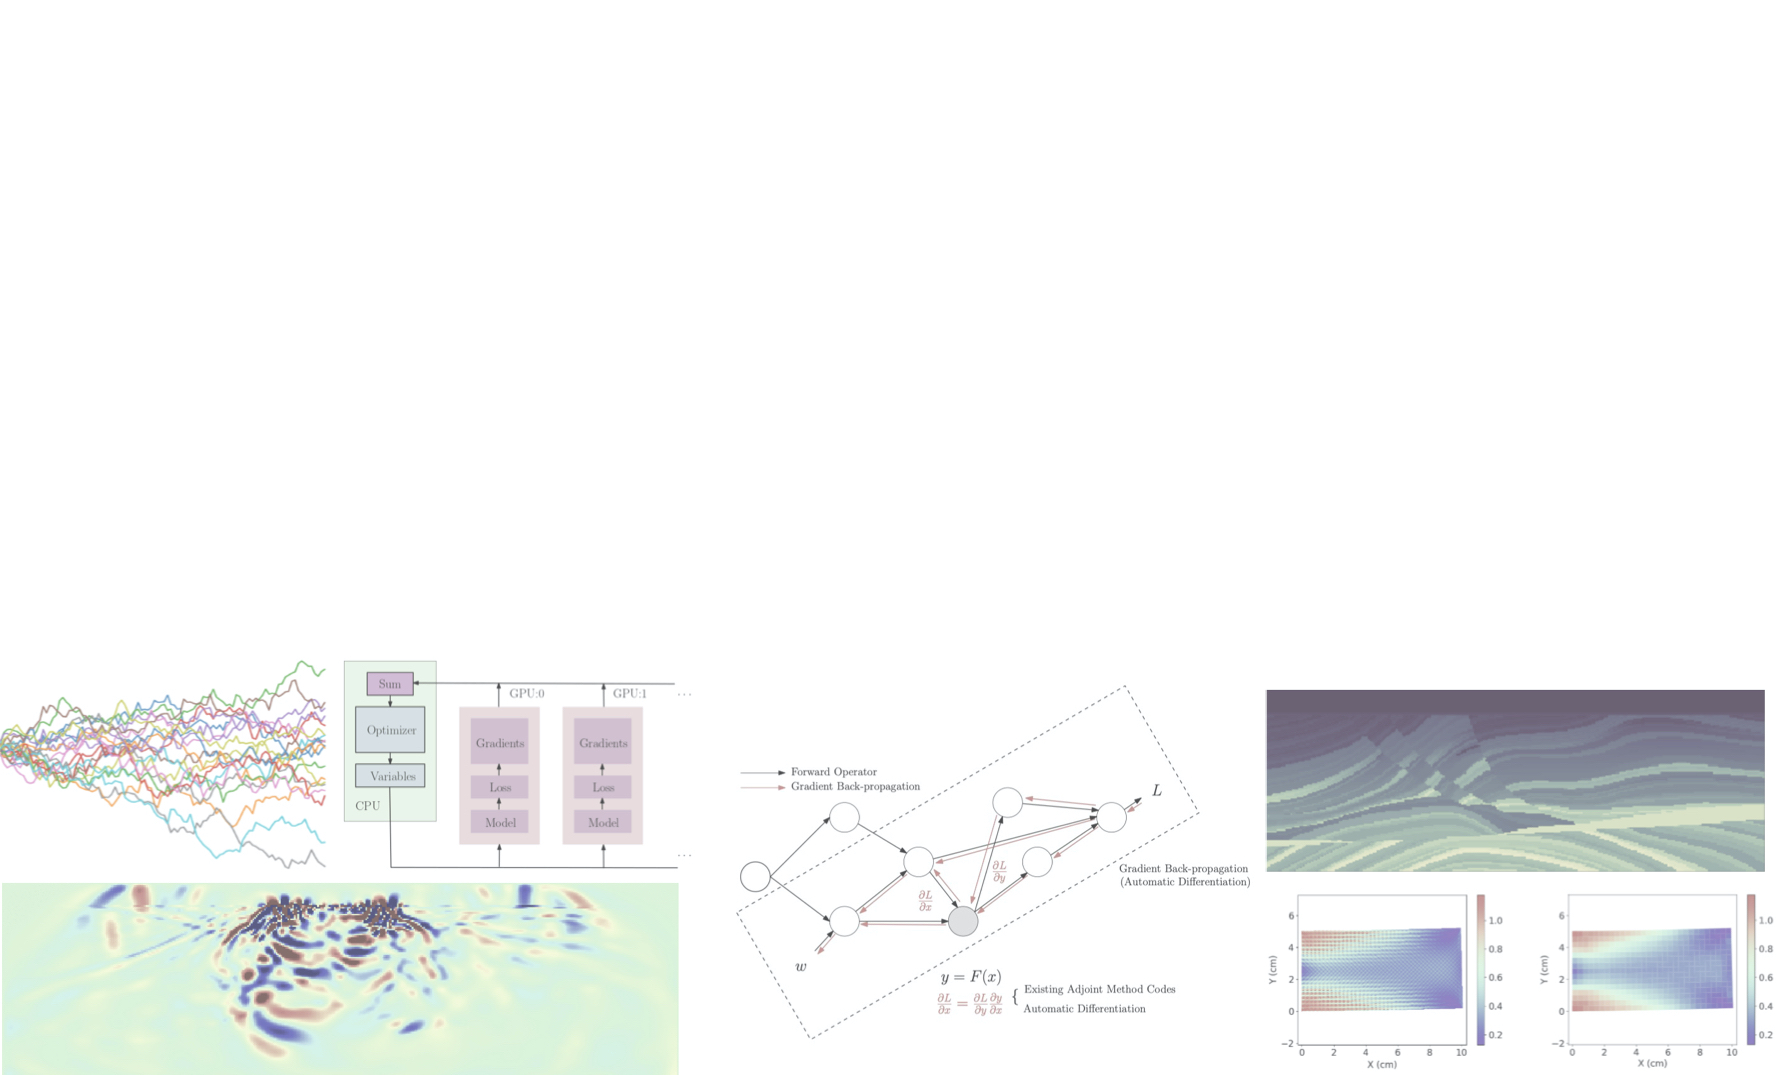
\includegraphics[width=1.0\paperwidth]{figures/background}}}
\end{picture}
  } 
%\usebackgroundtemplate{%
%  \includegraphics[width=\paperwidth,height=\paperheight]{figures/back}} 
\begin{frame}

\titlepage % Print the title page as the first slide

%dfa
\end{frame}
\usebackgroundtemplate{}

\section{Inverse Modeling}




\begin{frame}
	\frametitle{Inverse Modeling}
	\begin{figure}
	\centering
  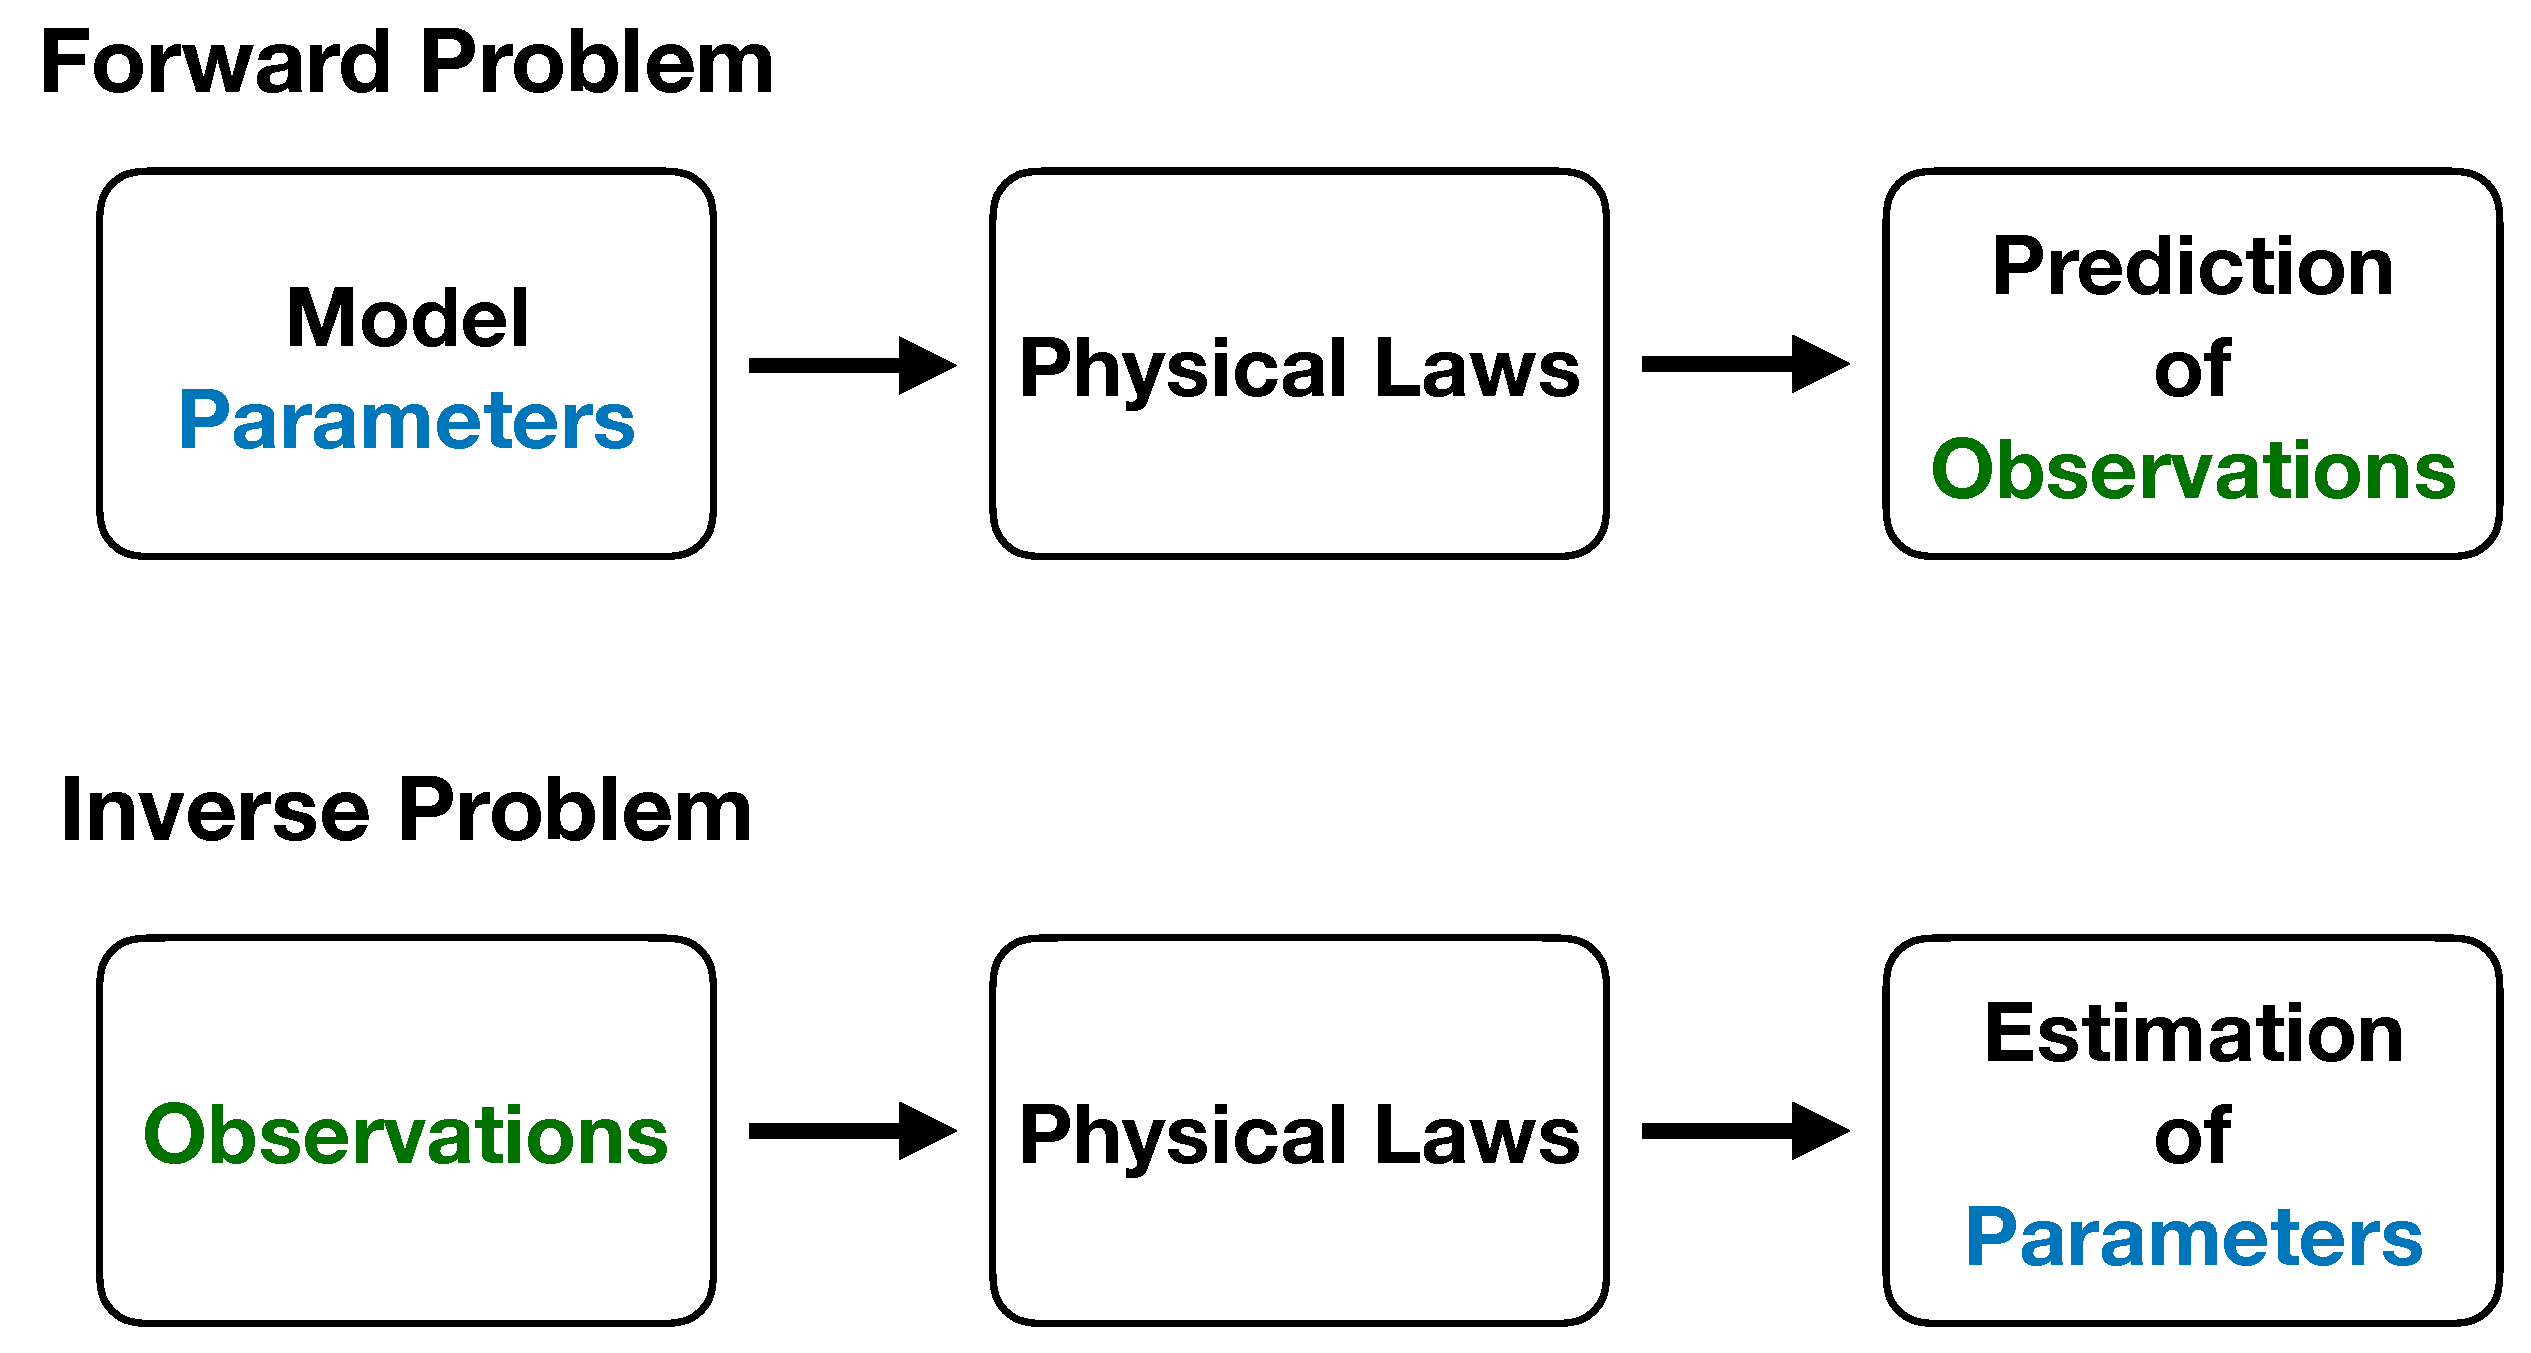
\includegraphics[width=1.0\textwidth]{figures/inverse3}
\end{figure}
\end{frame}

\begin{frame}
	\frametitle{Inverse Modeling}
	We can formulate inverse modeling as a PDE-constrained optimization problem 
	\begin{equation*}
		\min_{\theta} L_h(u_h) \quad \mathrm{s.t.}\; F_h(\theta, u_h) = 0
	\end{equation*}
	\begin{itemize}
		\item The \textcolor{red}{loss function} $L_h$ measures the discrepancy between the prediction $u_h$ and the observation $u_{\mathrm{obs}}$, e.g., $L_h(u_h) = \|u_h - u_{\mathrm{obs}}\|_2^2$. 
		\item $\theta$ is the \textcolor{red}{model parameter} to be calibrated. 
		\item The \textcolor{red}{physics constraints} $F_h(\theta, u_h)=0$ are described by a system of partial differential equations. Solving for $u_h$ may require solving linear systems or applying an iterative algorithm such as the Newton-Raphson method. 
	\end{itemize}
\end{frame}

\begin{frame}
	\frametitle{Function Inverse Problem}
	
	\begin{equation*}
		\min_{\textcolor{red}{f}} L_h(u_h) \quad \mathrm{s.t.}\; F_h(\textcolor{red}{f}, u_h) = 0
	\end{equation*}
	
	What if the unknown is a \textcolor{red}{function} instead of a set of parameters?
\begin{itemize}
	\item Koopman operator in dynamical systems.
	\item Constitutive relations in solid mechanics. 
	\item Turbulent closure relations in fluid mechanics.
	\item ...
\end{itemize}

The candidate solution space is \textcolor{red}{infinite dimensional}.

\end{frame}

\begin{frame}
	\frametitle{Machine Learning for Computational Engineering}
	$$\min_{\theta} L_h(u_h) \quad \mathrm{s.t.}\;F_h(\textcolor{red}{NN_\theta}, u_h) = 0$$
	\vspace{-0.5cm}
	\begin{itemize}
		\item Deep neural networks exhibit capability of approximating high dimensional and complicated functions. 
		\item \textbf{Physics based machine learning}: \textcolor{red}{the unknown function is approximated by a deep neural network, and the physical constraints are enforced by numerical schemes}.
		\item \textcolor{red}{Satisfy the physics to the largest extent}.
	\end{itemize}
	\begin{figure}[hbt]
  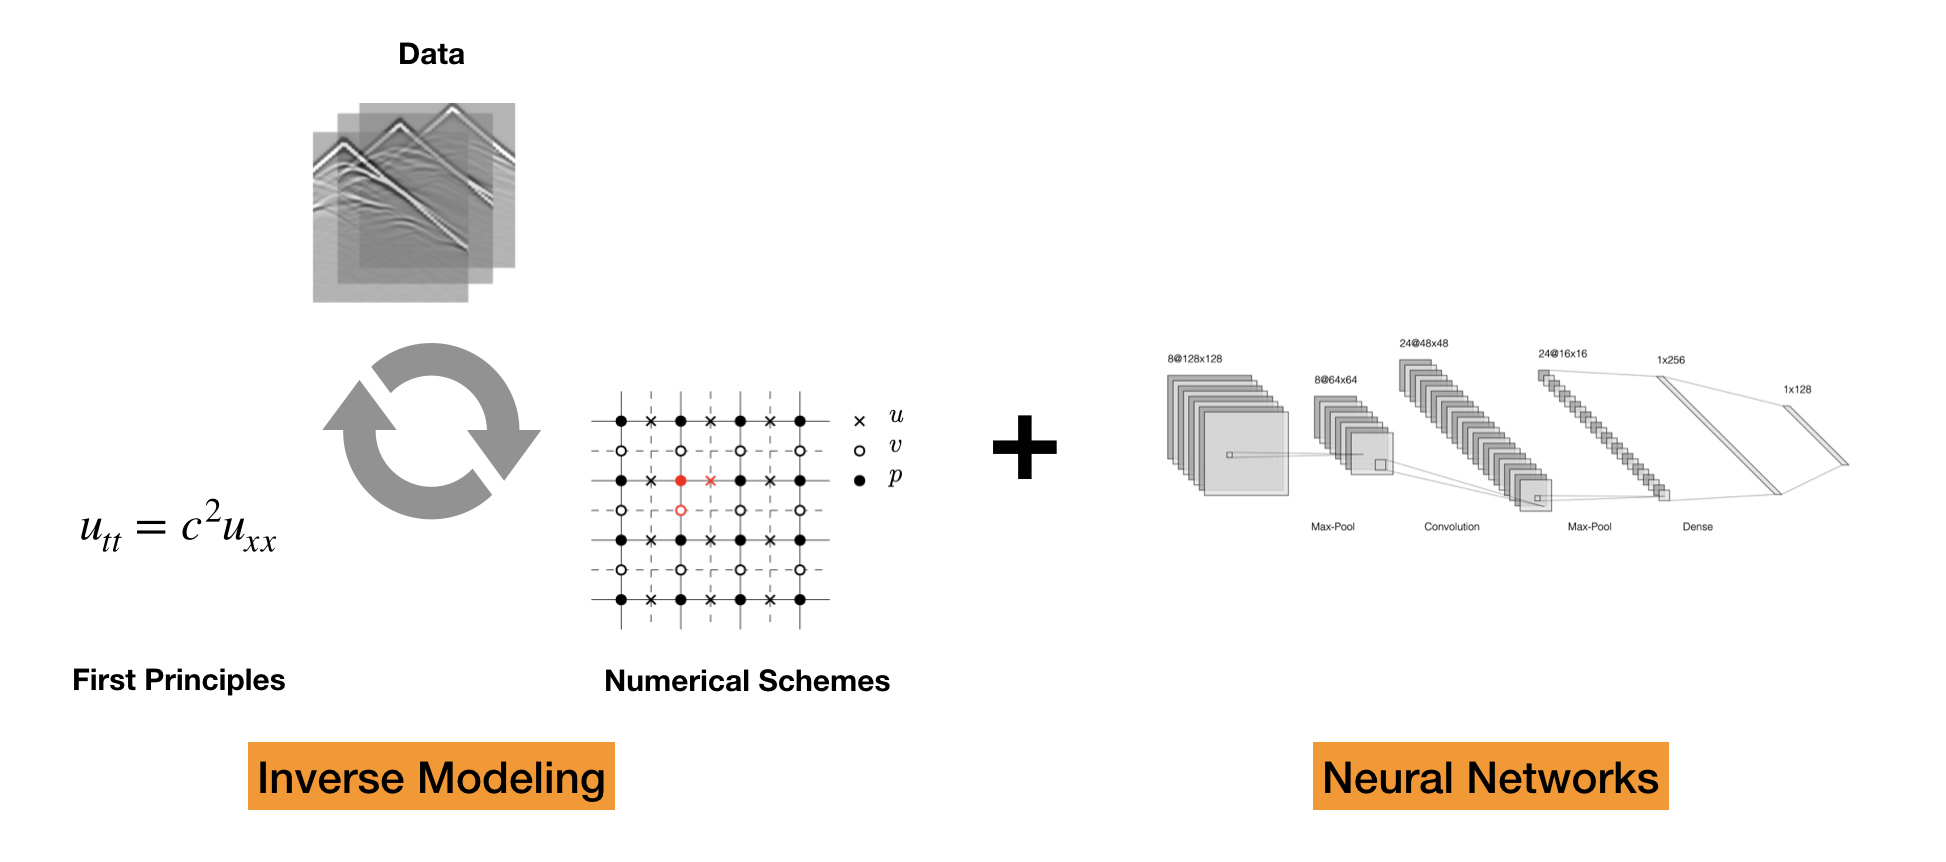
\includegraphics[width=0.75\textwidth]{figures/physics_based_machine_learning.png}
\end{figure}
\end{frame}



\begin{frame}
	\frametitle{Gradient Based Optimization}
	\begin{equation}\label{equ:opt}
		\min_{\theta} L_h(u_h) \quad \mathrm{s.t.}\; F_h(\theta, u_h) = 0
		\end{equation}
	
	\begin{itemize}
		\item We can now apply a gradient-based optimization method to (\ref{equ:opt}).
		\item The key is to \textcolor{red}{calculate the gradient descent direction} $g^k$
		$$\theta^{k+1} \gets \theta^k - \alpha g^k$$ 
	\end{itemize}
	
	\begin{figure}[hbt]
	\centering
  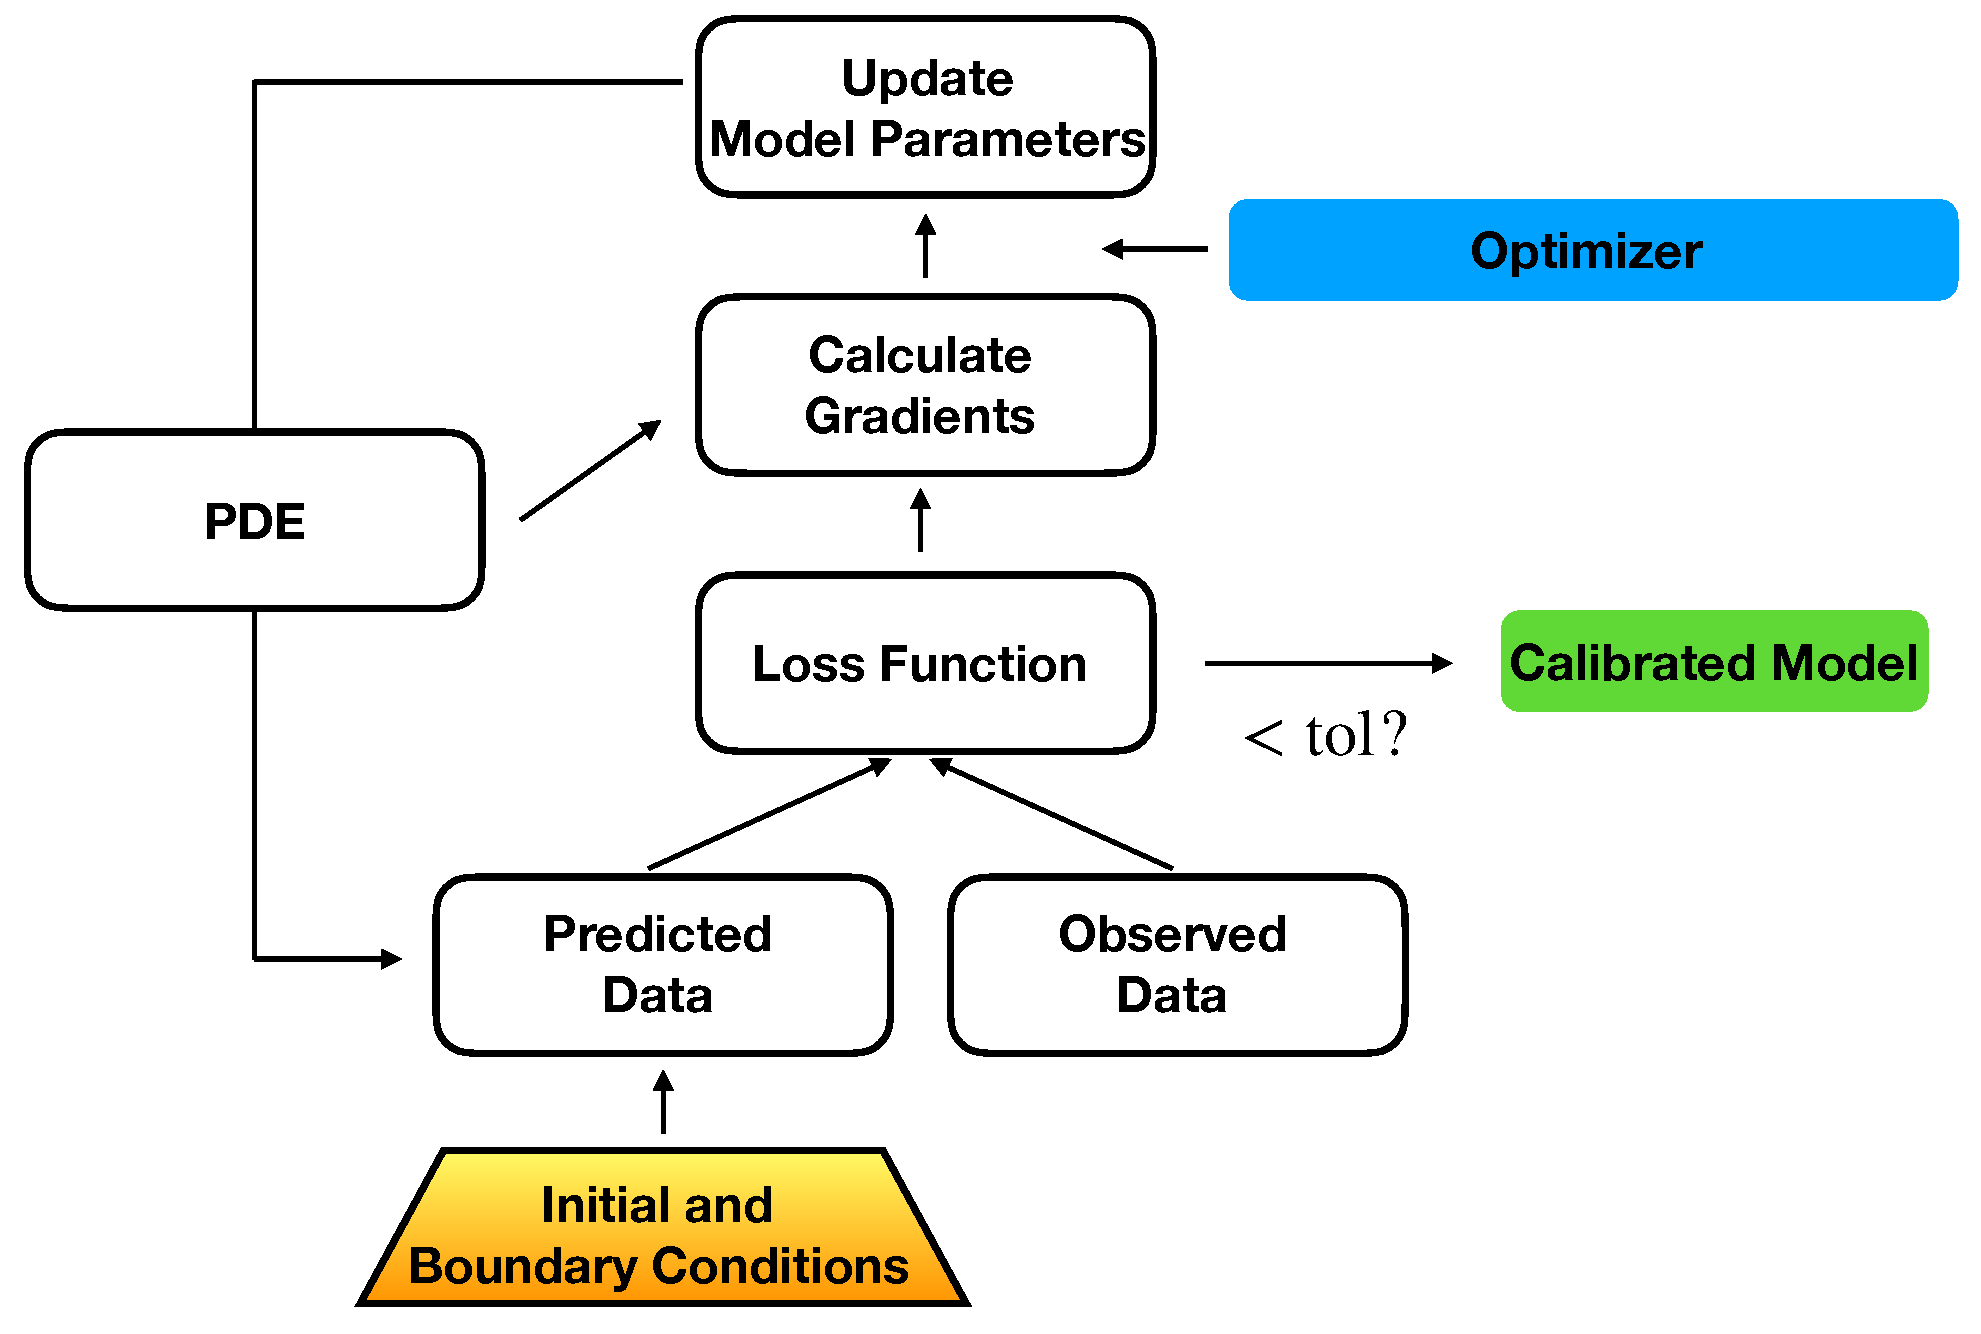
\includegraphics[width=0.6\textwidth]{figures/im.pdf}
\end{figure}

\end{frame}



\section{Automatic Differentiation}

\begin{frame}
	\frametitle{Automatic Differentiation}
The fact that bridges the \textcolor{red}{technical} gap between machine learning and inverse modeling:
	\begin{itemize}
		\item Deep learning (and many other machine learning techniques) and numerical schemes share the same computational model: composition of individual operators. 
	\end{itemize}
	

\begin{minipage}[t]{0.4\textwidth}

\



\begin{center}
			\textcolor{red}{Mathematical Fact}

			\
			
	Back-propagation 

$||$

Reverse-mode

 Automatic Differentiation 

$||$
 
 Discrete 
 
 Adjoint-State Method
\end{center}
\end{minipage}~
\begin{minipage}[t]{0.6\textwidth}
\begin{figure}[hbt]
  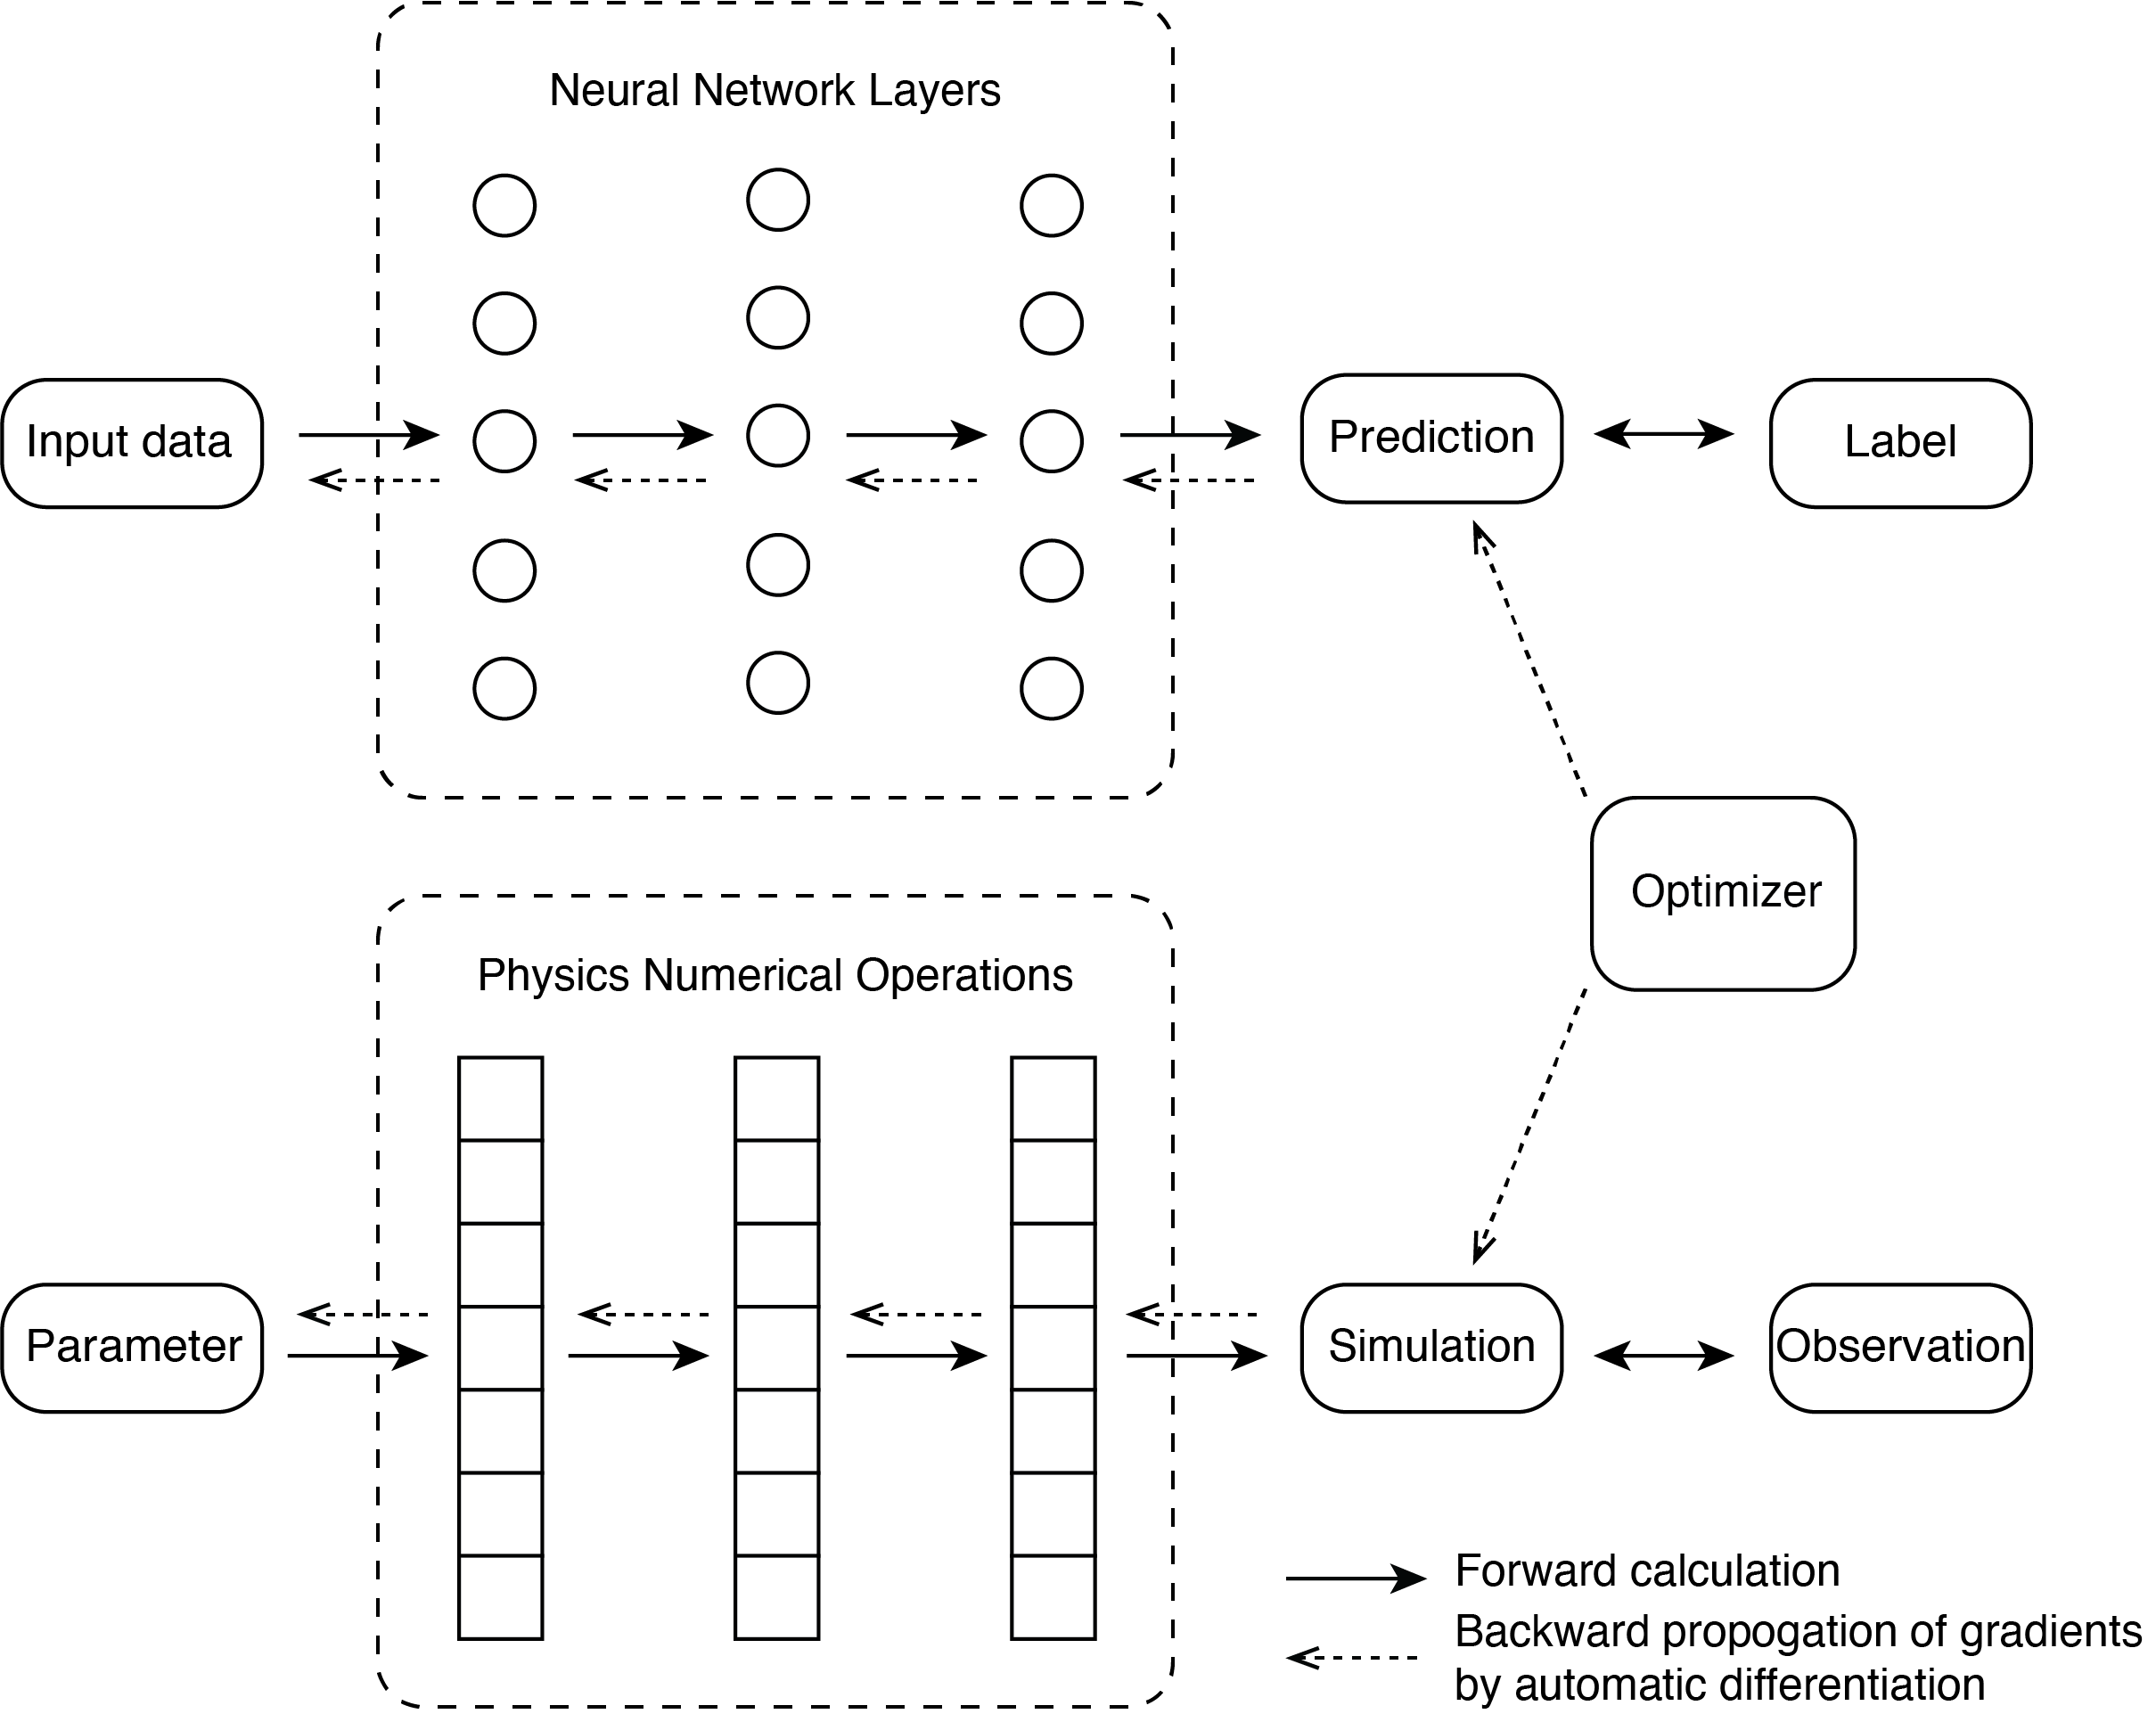
\includegraphics[width=0.8\textwidth]{figures/compare-NN-PDE.png}
\end{figure}
\end{minipage}

\end{frame}


\begin{frame}
	\frametitle{Automatic Differentiation: Computational Graph}
	
	\begin{itemize}
		\item A computational graph is a functional description of the required computation. In the computational graph, an edge represents \textcolor{red}{data}, such as a scalar, a vector, a matrix or a tensor. A node represents a \textcolor{red}{function (operator)} whose input arguments are the the incoming edges and output values are are the outcoming edges. 
		\item How to build a computational graph for $z = \sin(x_1+x_2) + x_2^2 x_3$?
	\end{itemize}
	
	\begin{figure}[hbt]
  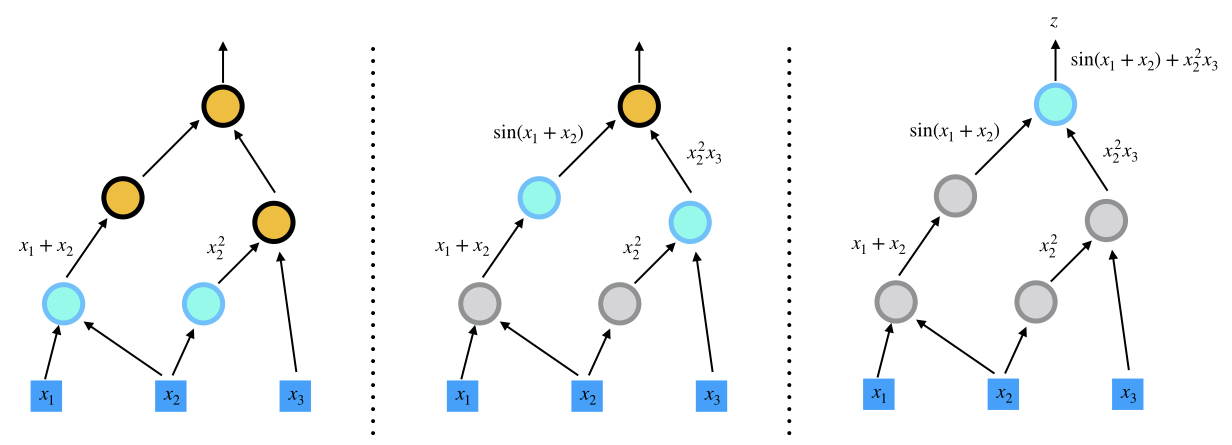
\includegraphics[width=1.0\textwidth]{figures/fd}
\end{figure}
\end{frame}

\begin{frame}
	\frametitle{Reverse Mode AD}
	$$\frac{df(g(x))}{dx} = \red{f'(g(x))} g'(x)$$
	\begin{itemize}
		\item Computing in the reverse order of forward computation. 
		\item Each node in the computational graph
		\begin{itemize}
		\item \red{Aggregates} all the gradients from down-streams 
		\item \red{Back-propagates} the gradient to upstream nodes.  
		\end{itemize}
		\begin{figure}[hbt]
  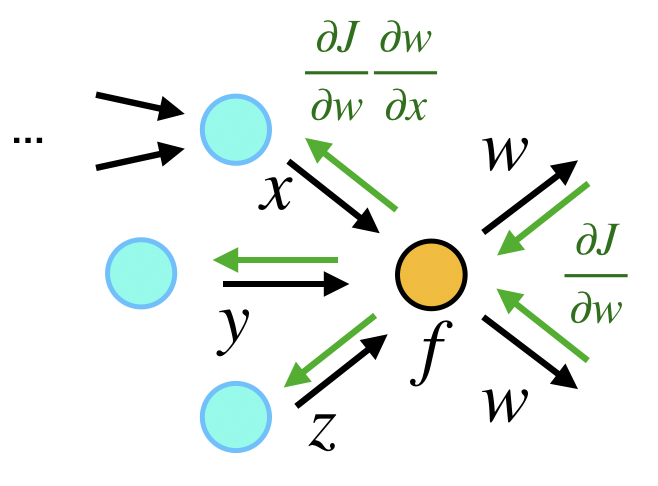
\includegraphics[width=0.4\textwidth]{figures/rad}
\end{figure}

	\end{itemize}
\end{frame}


\begin{frame}
\frametitle{Example: Reverse Mode AD}	
$$z=\sin(x_1+x_2) + x_2^2x_3$$
\begin{figure}[hbt]
\centering
  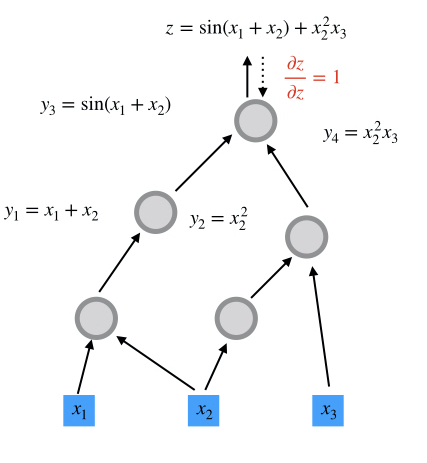
\includegraphics[width=0.5\textwidth]{figures/bd1}
\end{figure}

  
\end{frame}

\begin{frame}
\frametitle{Example: Reverse Mode AD}	
$$z=\sin(x_1+x_2) + x_2^2x_3$$
\begin{figure}[hbt]
\centering
  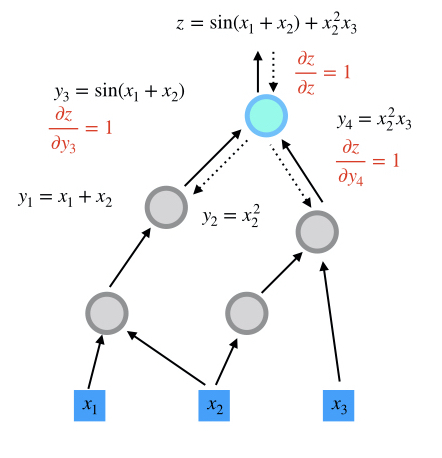
\includegraphics[width=0.5\textwidth]{figures/bd2}
\end{figure}
\end{frame}


\begin{frame}
\frametitle{Example: Reverse Mode AD}	
$$z=\sin(x_1+x_2) + x_2^2x_3$$
\begin{figure}[hbt]
\centering
  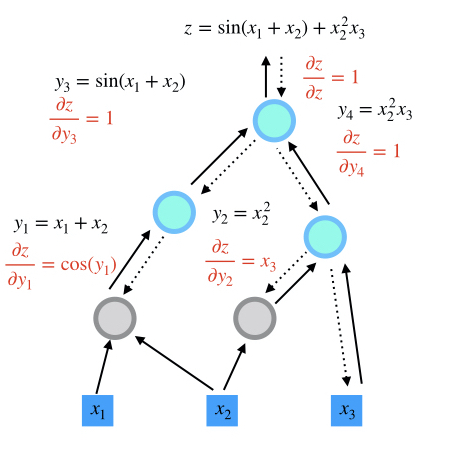
\includegraphics[width=0.5\textwidth]{figures/bd3}
\end{figure}
\end{frame}

\begin{frame}
\frametitle{Example: Reverse Mode AD}	
$$z=\sin(x_1+x_2) + x_2^2x_3$$
\begin{figure}[hbt]
\centering
  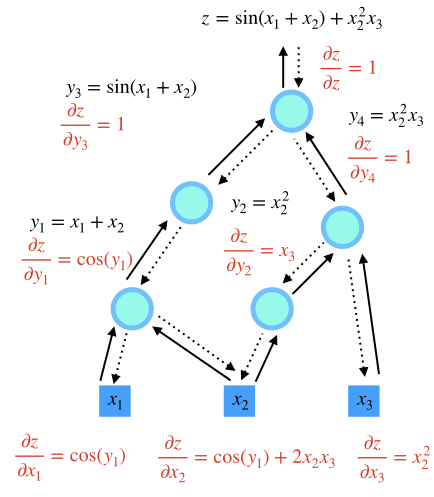
\includegraphics[width=0.5\textwidth]{figures/bd4}
\end{figure}
\end{frame}

\begin{frame}
	\frametitle{Forward Mode AD}

	\begin{itemize}
	\item The forward-mode automatic differentiation uses the chain rule to propagate the gradients. 
	$$\frac{\partial f\circ g (x)}{\partial x} =  f'(g(x)) \red{ g'(x)}$$
		\item Compute in the same order as function evaluation. 
		\item Each node in the computational graph
		\begin{itemize}
		\item \red{Aggregate} all the gradients from up-streams. 
		\item \red{Forward} the gradient to down-stream nodes.  
		\end{itemize} 
	\end{itemize}
	
	\begin{figure}[hbt]
  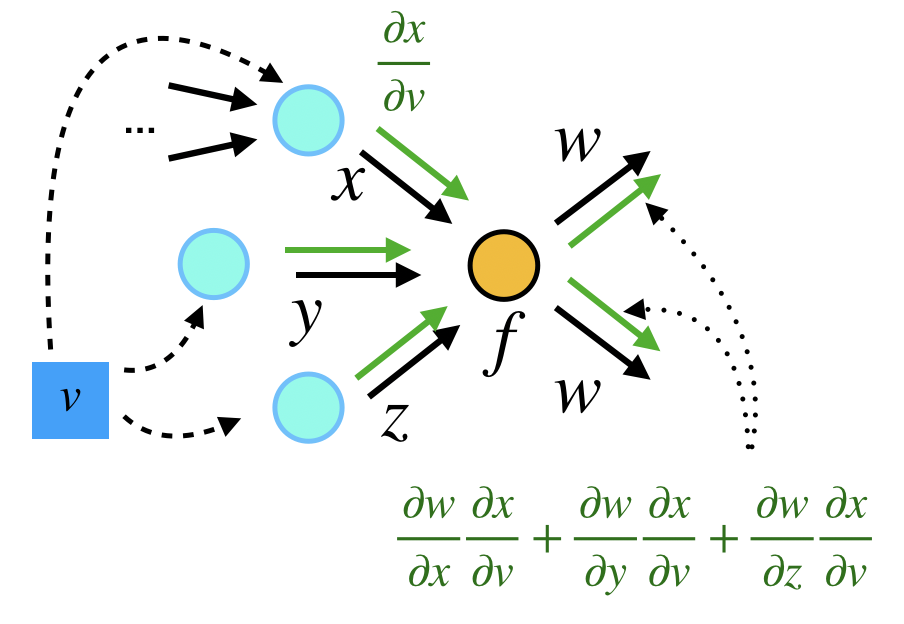
\includegraphics[width=0.4\textwidth]{figures/fad}
\end{figure}
	
	
\end{frame}

\begin{frame}
	\frametitle{Example: Forward Mode AD}
	\begin{itemize}
	\item 	Let's consider a specific way for computing 
	\begin{equation*}
		f(x) = \begin{bmatrix}
			x^4\\
			x^2 + \sin(x) \\
			-\sin(x)
		\end{bmatrix}
	\end{equation*}
	\end{itemize}

	
	
	\begin{minipage}[b]{0.45\textwidth}
	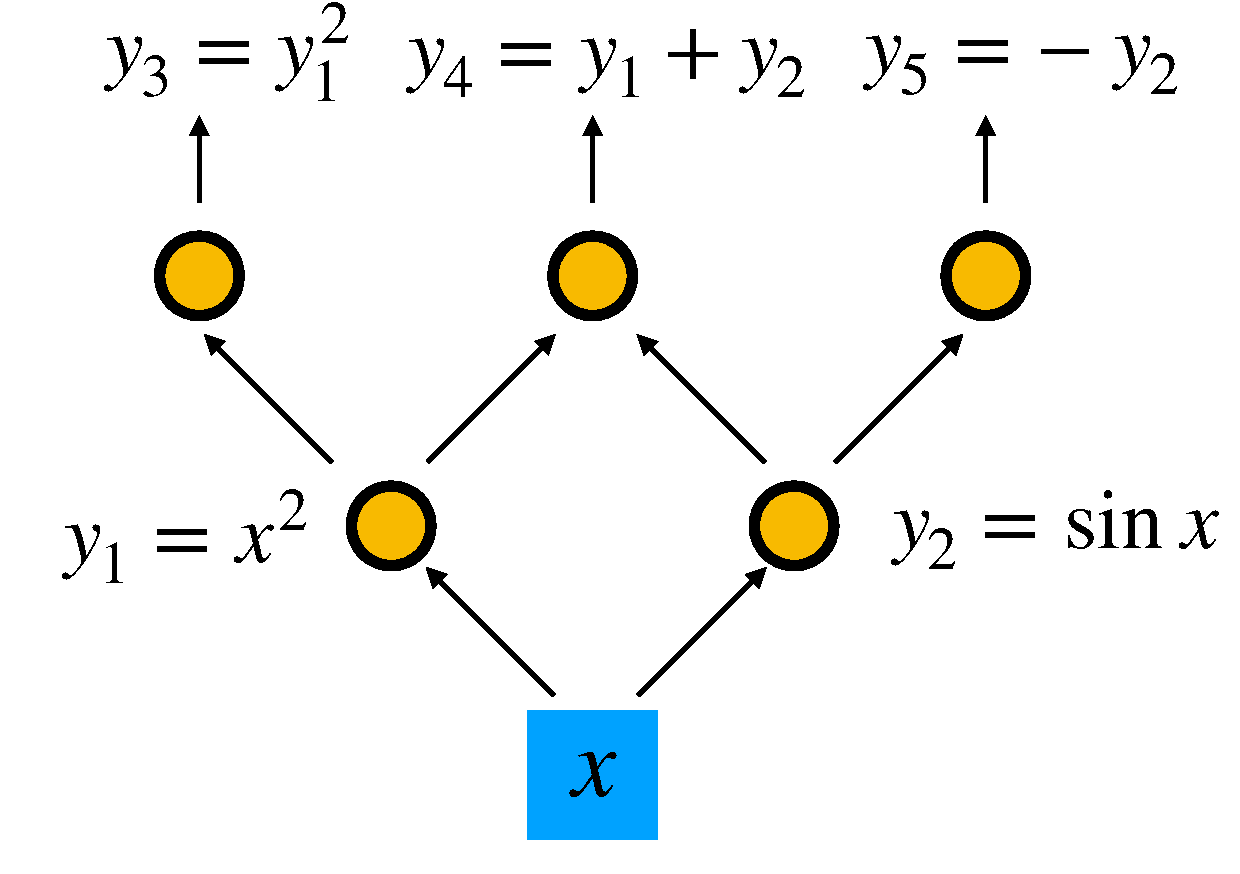
\includegraphics[width=1.0\textwidth]{figures/forwardmode}
\end{minipage}~
\begin{minipage}[b]{0.45\textwidth}
  \begin{align*}
(y_1, y_1')& = (x^2, 2x) \\
(y_2, y_2') &= (\sin x, \cos x) \\
\\
(y_3, y_3') &= (y_1^2, 2y_1y_1') = (x^4, 4x^3)\\
(y_4, y_4') &= (y_1+y_1, y_1'+y_2') \\
&= (x^2+\sin x, 2x+\cos x) \\
(y_5, y_5')& = (-y_2, -y_2') = (-\sin x, -\cos x)
 	\end{align*}
\end{minipage}
\end{frame}


\begin{frame}
	\frametitle{Summary}
	
	\begin{itemize}
		\item In general, for a function $f:\RR^n \rightarrow \RR^m$
		 % Please add the following required packages to your document preamble:
% \usepackage{booktabs}
\begin{table}[]
\centering
\begin{tabular}{@{}llll@{}}
\toprule
Mode & Suitable for ... & Complexity\footnote{$\mathrm{OPS}$ is a metric for complexity in terms of fused-multiply adds.} & Application \\ \midrule
Forward & $m\gg n$ & $\leq 2.5\;\mathrm{OPS}(f(x))$ & UQ \\
Reverse & $m\ll n$ & $\leq 4\;\mathrm{OPS}(f(x))$ & Inverse Modeling \\ \bottomrule
\end{tabular}
\end{table}
	
		
		\item There are also many other interesting topics
		\begin{itemize}
		\item Mixed mode AD: many-to-many mappings.
		\item Computing sparse Jacobian matrices using AD by exploiting sparse structures. 
		\end{itemize}
	\end{itemize}
	{\scriptsize Margossian CC. A review of automatic differentiation and its efficient implementation. Wiley Interdisciplinary Reviews: Data Mining and Knowledge Discovery. 2019 Jul;9(4):e1305.} 
\end{frame}

\begin{frame}
	\frametitle{Computational Graph for Numerical Schemes}
	
	\begin{itemize}
		\item To leverage automatic differentiation for inverse modeling, we need to express the numerical schemes in the ``AD language'': computational graph. 
		\item No matter how complicated a numerical scheme is, it can be decomposed into a collection of operators that are interlinked via state variable dependencies. 
	\end{itemize}
	
	\begin{figure}[hbt]
  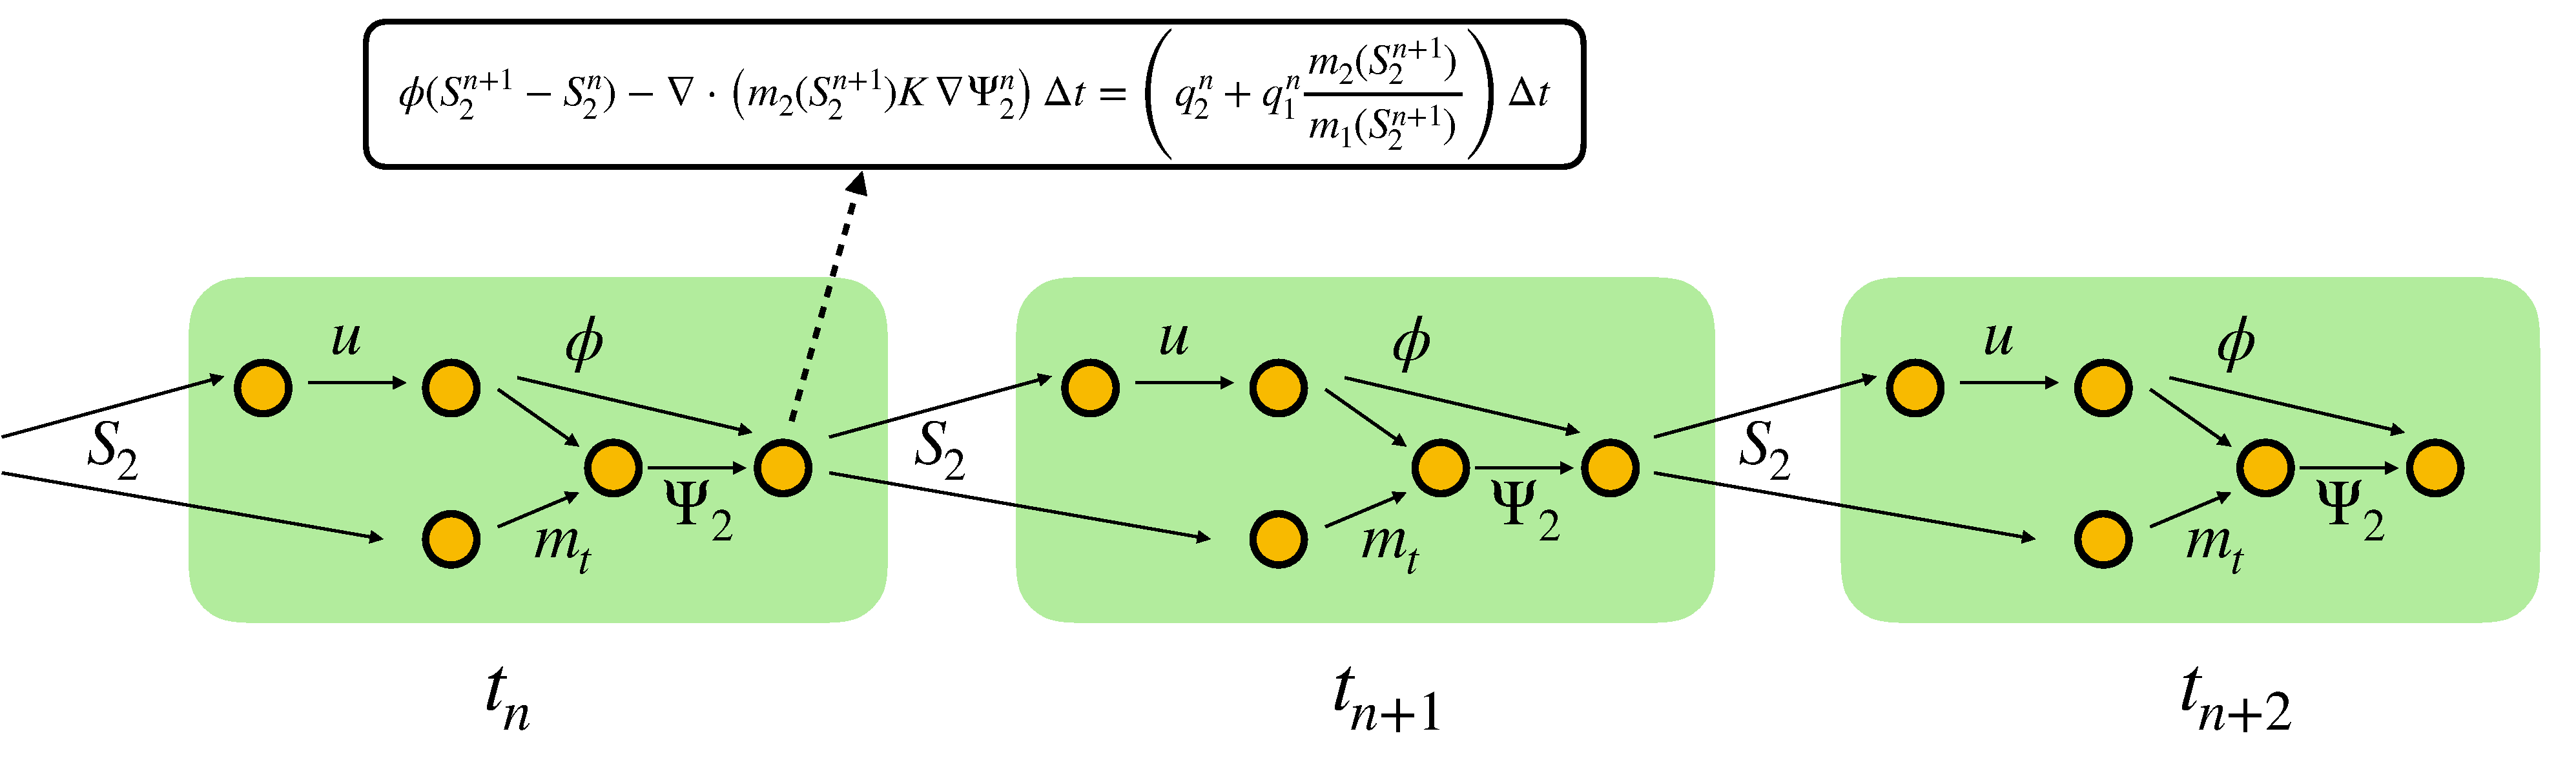
\includegraphics[width=1.0\textwidth]{figures/cgnum}
\end{figure}

	
	
\end{frame}

\begin{frame}
	\frametitle{The  Relationship between reverse-mode Automatic Differentiation and KKT Condition}
	Consider a concrete PDE-constrained optimization problem:
	
	\begin{minipage}[b]{0.45\textwidth}
		\begin{align*}
     \min_{\mathbf{u}_1, \bm{\theta}} &\  J = f_4(\mathbf{u}_1, \mathbf{u}_2, \mathbf{u}_3, \mathbf{u}_4), \\
     \mathrm{s.t.} & \ \mathbf{u}_2 = f_1(\mathbf{u}_1, \bm {\theta}), \\
     & \ \mathbf{u}_3 = f_2(\mathbf{u}_2, \bm {\theta}),\\
     & \  \mathbf{u}_4 = f_3(\mathbf{u}_3, \bm {\theta}).
\end{align*}
-- $f_1$, $f_2$, $f_3$ are PDE constraints

-- $f_4$ is the loss function

-- $\bu_1$ is the initial condition

-- $\bt$ is the model parameter
	\end{minipage}~
	\begin{minipage}[b]{0.45\textwidth}
		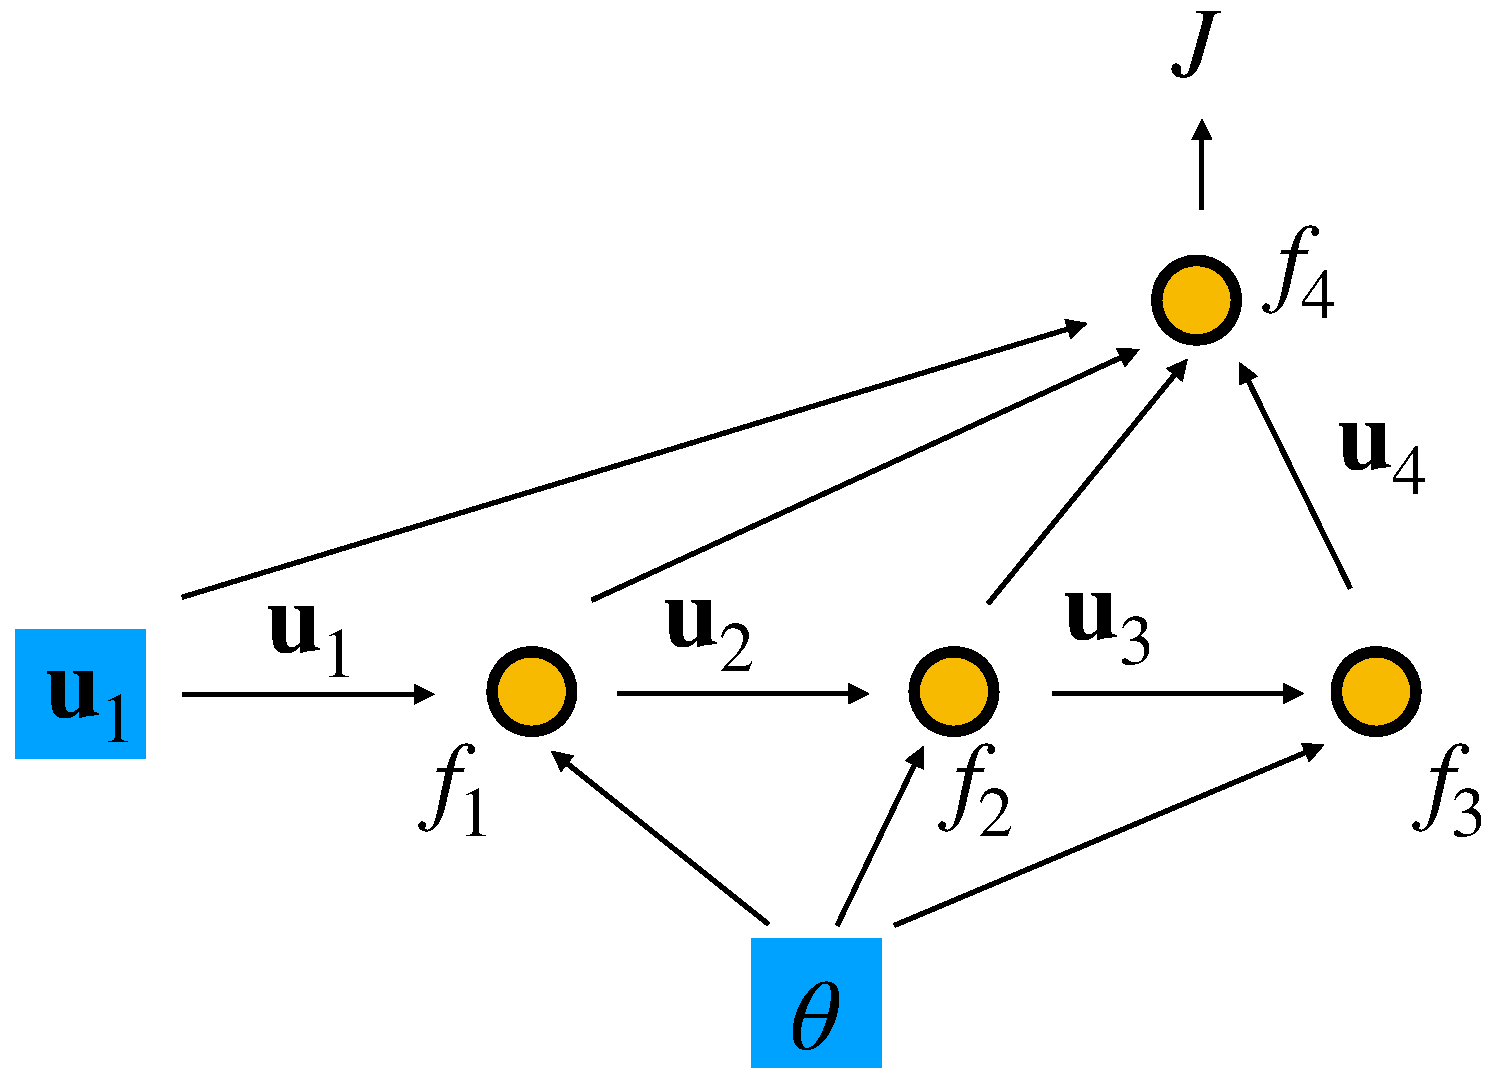
\includegraphics[width=1.0\textwidth]{figures/adjoint}
	\end{minipage}
	 
	
	
	
	\end{frame}
	


\begin{frame}
	\frametitle{Granularity of Automatic Differentiation}
	
	
	\begin{figure}[hbt]
		\centering
		\includegraphics[width=0.8\textwidth]{figures/adlevel}
	\end{figure}
	
	
	
\end{frame}


\begin{frame}
	\frametitle{Inverse Modeling of the Stokes Equation}
	
	\begin{itemize}
		\item The governing equation for the Stokes problem
			$$\begin{aligned} -\textcolor{red}{\nu}\Delta \mathbf{u} + \nabla p &= \mathbf{f} & \text{ in } \Omega \\ \nabla \cdot \mathbf{u} &= 0 & \text{ in } \Omega \\ \mathbf{u} &= \mathbf{0} & \text{ on } \partial \Omega \end{aligned}$$
	\end{itemize}


\begin{minipage}[c]{0.7\textwidth}
\begin{itemize}
	\item The weak form is given by 
	\begin{equation*}
		\begin{aligned}
			(\textcolor{red}{\nu} \nabla u, \nabla v) &- (p, \nabla \cdot v) &&= (f, v)\\
			(\nabla \cdot u, q) & &&= 0
		\end{aligned}
	\end{equation*}
\end{itemize}
\end{minipage}~
\begin{minipage}[c]{0.29\textwidth}
	\includegraphics[width=1.0\textwidth]{figures/stokesuvp}
\end{minipage}



	
	
\end{frame}


\begin{frame}[fragile]{}
	\frametitle{Inverse Modeling of the Stokes Equation}
	
	\begin{minted}[escapeinside=||,fontsize=\small]{julia}
|\textbf{\colorbox{green}{nu = \texttt{Variable(0.5)}}}|
K = nu*constant(|\underline{\texttt{compute\_fem\_laplace\_matrix}}|(m, n, h))
B = constant(|\underline{\texttt{compute\_interaction\_matrix}}|(m, n, h))
Z = [K -B'
    -B spdiag(zeros(size(B,1)))]

# Impose boundary conditions
bd = bcnode("all", m, n, h)
bd = [bd; bd .+ (m+1)*(n+1); ((1:m) .+ 2(m+1)*(n+1))]
Z, _ = |\underline{\texttt{fem\_impose\_Dirichlet\_boundary\_condition1}}|(Z, bd, m, n, h)

# Calculate the source term 
F1 = |\underline{\texttt{eval\_f\_on\_gauss\_pts}}|(f1func, m, n, h)
F2 = |\underline{\texttt{eval\_f\_on\_gauss\_pts}}|(f2func, m, n, h)
F = |\underline{\texttt{compute\_fem\_source\_term}}|(F1, F2, m, n, h)
rhs = [F;zeros(m*n)]
rhs[bd] .= 0.0

sol = Z\rhs 
	\end{minted}
	
	
\end{frame}



\begin{frame}[fragile]{}
	\frametitle{Inverse Modeling of the Stokes Equation}
	
	\begin{itemize}
		\item The distinguished feature compared to traditional forward simulation programs: \textcolor{red}{the model output is differentiable with respect to model parameters}!
		\begin{minted}[escapeinside=||,fontsize=\small]{julia}
loss = sum((sol[idx] - observation[idx])^2)
g = gradients(loss, nu)
		\end{minted}
		\item Optimization with a one-liner:
\begin{minted}[escapeinside=||,fontsize=\small]{julia}
BFGS!(sess, loss)
\end{minted}	 
	\end{itemize}

	\begin{figure}[hbt]
	\centering
	\includegraphics[width=0.8\textwidth]{figures/lego}
\end{figure}
	
\end{frame}


%\begin{frame}
%	\frametitle{Code Example}
%	\begin{itemize}
%		\item  Find $b$ such that $u(0.5)=1.0$ and
%		$$-bu''(x)+u(x) = 8 + 4x - 4x^2, x\in[0,1], u(0)=u(1)=0$$
%	\end{itemize}
%	\begin{figure}[hbt]
%  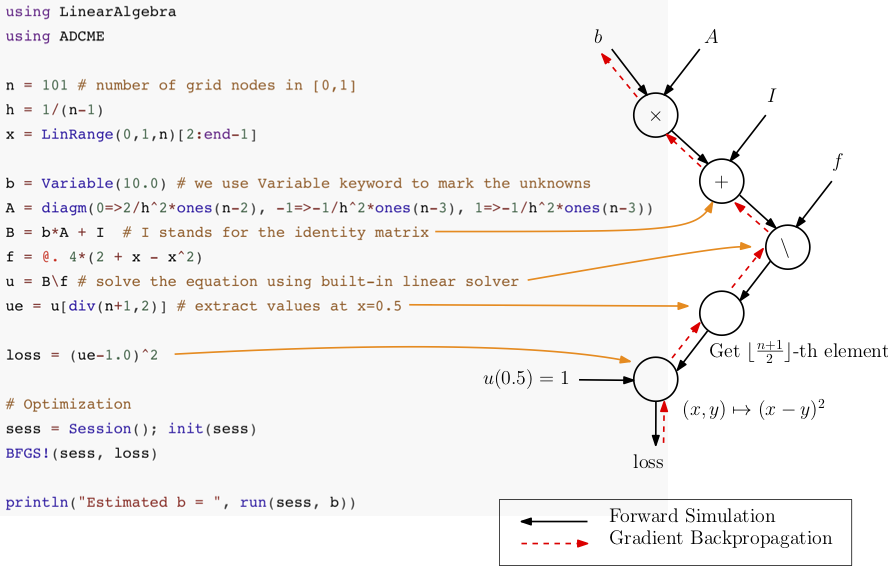
\includegraphics[width=0.8\textwidth]{figures/code.png}
%\end{figure}
%\end{frame}


\section{Physics Constrained Learning}
\begin{frame}


	\frametitle{Challenges in AD}
	
	
	\begin{minipage}[t]{0.49\textwidth}
	\vspace{-3cm}
\begin{itemize}
	\item Most AD frameworks only deal with explicit operators, i.e., the functions that has analytical derivatives, or composition of these functions. 
	\item Many scientific computing algorithms are \textcolor{red}{iterative} or \textcolor{red}{implicit} in nature.
\end{itemize}
\end{minipage}~
\begin{minipage}[t]{0.49\textwidth}
  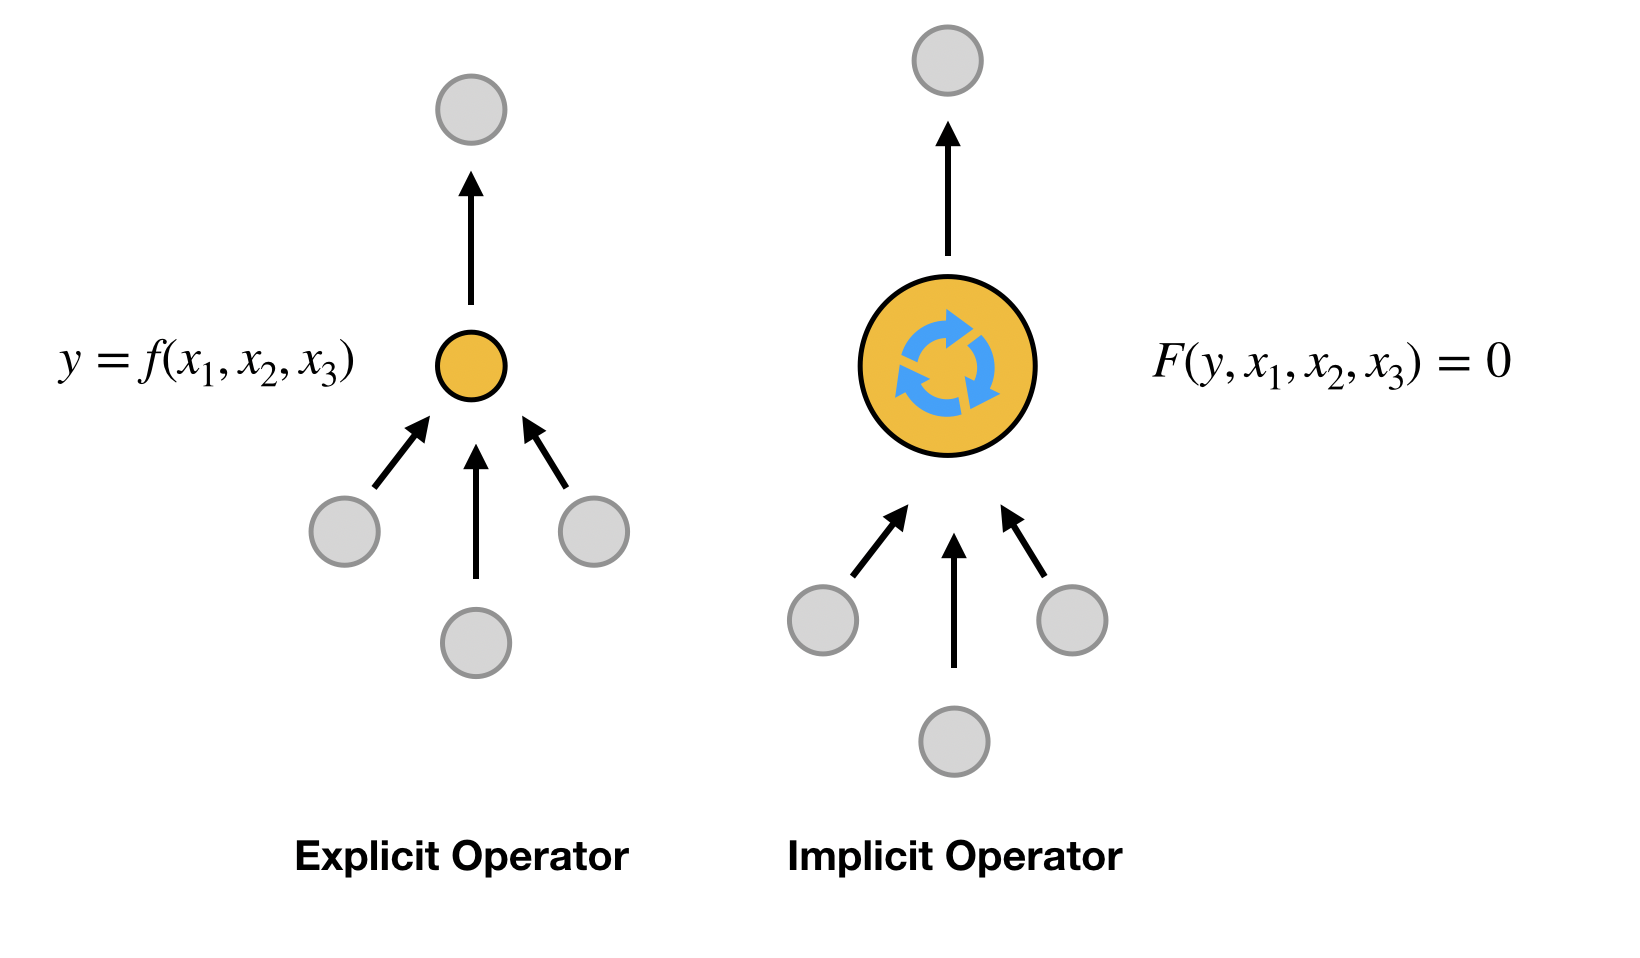
\includegraphics[width=1.0\textwidth]{figures/sim.png}
\end{minipage}

	% Please add the following required packages to your document preamble:
% \usepackage{booktabs}
\begin{table}[]
\begin{tabular}{@{}lll@{}}
\toprule
Linear/Nonlinear & Explicit/Implicit & Expression   \\ \midrule
Linear           & Explicit          & $y=Ax$       \\
Nonlinear        & Explicit          & $y = F(x)$   \\
\textbf{Linear}           & \textbf{Implicit}          & $Ay = x$     \\
\textbf{Nonlinear}        & \textbf{Implicit}          & $F(x,y) = 0$ \\ \bottomrule
\end{tabular}
\end{table}
\end{frame}

\begin{frame}
	\frametitle{Example}

	\begin{itemize}
		%		\item A simple approach is to save part or all intermediate steps, and ``back-propagate''. This approach is expensive in both computation and memory\footnote{Ablin, Pierre, Gabriel Peyr�, and Thomas Moreau. ``Super-efficiency of automatic differentiation for functions defined as a minimum.''}.
		%		\item Nevertheless, the simple approach works in some scenarios where accuracy or cost is not an issue, e.g., automatic differetiation of soft-DTW and Sinkhorn distance. 
		\item An efficient way to do automatic differentiation is to apply the \textcolor{red}{implicit function theorem}. For our example, $F(x,y)=x^3-(y^3+y)=0$; treat $y$ as a function of $x$ and take the derivative on both sides
		      $$3x^2 - 3y(x)^2y'(x)-y'(x)=0\Rightarrow y'(x) = \frac{3x^2}{3y^2+1}$$
		      The above gradient is \textcolor{red}{exact}.
	\end{itemize}
	\begin{center}
		\textbf{Can we apply the same idea to inverse modeling?}
	\end{center}

\end{frame}

\begin{frame}
	\frametitle{Example}
	
	\begin{itemize}
%		\item A simple approach is to save part or all intermediate steps, and ``back-propagate''. This approach is expensive in both computation and memory\footnote{Ablin, Pierre, Gabriel Peyré, and Thomas Moreau. ``Super-efficiency of automatic differentiation for functions defined as a minimum.''}.
%		\item Nevertheless, the simple approach works in some scenarios where accuracy or cost is not an issue, e.g., automatic differetiation of soft-DTW and Sinkhorn distance. 
		\item An efficient way is to apply the \textcolor{red}{implicit function theorem}. For our example, $F(x,y)=x^3-(y^3+y)=0$, treat $y$ as a function of $x$ and take the derivative on both sides
		$$3x^2 - 3y(x)^2y'(x)-1=0\Rightarrow y'(x) = \frac{3x^2-1}{3y(x)^2}$$
	The above gradient is \textcolor{red}{exact}.
	\end{itemize}
	\begin{center}
			\textbf{Can we apply the same idea to inverse modeling?}
	\end{center}

\end{frame}


\begin{frame}
	\frametitle{Physics Constrained Learning}
	$${\small    \min_{\theta}\; L_h(u_h) \quad \mathrm{s.t.}\;\; F_h(\theta, u_h) = 0}$$
	\begin{itemize}
		\item Assume that we solve for $u_h=G_h(\theta)$ with $F_h(\theta, u_h)=0$, and then
		      $${\small\tilde L_h(\theta)  = L_h(G_h(\theta))}$$
		\item Applying the \textcolor{red}{implicit function theorem}
		      {  \scriptsize
			      \begin{equation*}
				      \frac{{\partial {F_h(\theta, u_h)}}}{{\partial \theta }} + {\frac{{\partial {F_h(\theta, u_h)}}}{{\partial {u_h}}}}
				      \textcolor{red}{\frac{\partial G_h(\theta)}{\partial \theta}}
				      = 0 \Rightarrow
				      \textcolor{red}{\frac{\partial G_h(\theta)}{\partial \theta}} =  -\Big( \frac{{\partial {F_h(\theta, u_h)}}}{{\partial {u_h}}} \Big)^{ - 1} \frac{{\partial {F_h(\theta, u_h)}}}{{\partial \theta }}
			      \end{equation*}
		      }
		\item Finally we have
			      {\scriptsize
				      \begin{equation*}
					      \boxed{\frac{{\partial {{\tilde L}_h}(\theta )}}{{\partial \theta }}
					      = \frac{\partial {{ L}_h}(u_h )}{\partial u_h}\frac{\partial G_h(\theta)}{\partial \theta}=
					      - \textcolor{red}{ \frac{{\partial {L_h}({u_h})}}{{\partial {u_h}}} } \;
					      \textcolor{blue}{ \Big( {\frac{{\partial {F_h(\theta, u_h)}}}{{\partial {u_h}}}\Big|_{u_h = {G_h}(\theta )}} \Big)^{ - 1} } \;
					      \textcolor{ForestGreen}{ \frac{{\partial {F_h(\theta, u_h)}}}{{\partial \theta }}\Big|_{u_h = {G_h}(\theta )} }
					      }
				      \end{equation*}
			      }

	\end{itemize}

\end{frame}


\begin{frame}
	\frametitle{Physics Constrained Learning}
	{\scriptsize$$\boxed{\frac{{\partial {{\tilde L}_h}(\theta )}}{{\partial \theta }}
		= - \textcolor{red}{ \frac{{\partial {L_h}({u_h})}}{{\partial {u_h}}} } \;
		\textcolor{blue}{ \Big( {\frac{{\partial {F_h(\theta, u_h)}}}{{\partial {u_h}}}\Big|_{u_h = {G_h}(\theta )}} \Big)^{ - 1} } \;
		\textcolor{ForestGreen}{ \frac{{\partial {F_h(\theta, u_h)}}}{{\partial \theta }}\Big|_{u_h = {G_h}(\theta )} }
		}$$}

	Step 1: Calculate $w$ by solving a linear system (never invert the matrix!)
	{\scriptsize$$w^T = \underbrace{\frac{{\partial {L_h}({u_h})}}{{\partial {u_h}}\rule[-9pt]{1pt}{0pt}}}_{1\times N}
		\;\;
		\underbrace{\Big( {\frac{{\partial {F_h}}}{{\partial {u_h}}}\Big|_{u_h = {G_h}(\theta )}} \Big)^{ - 1}}_{N\times N}$$}
	Step 2: Calculate the gradient by automatic differentiation
	{\scriptsize$$w^T\;\underbrace{\frac{{\partial {F_h}}}{{\partial \theta }}\Big|_{u_h = {G_h}(\theta )}}_{N\times p} = \frac{\partial (w^T\;  {F_h}(\theta, u_h))}{\partial \theta }\Bigg|_{u_h = {G_h}(\theta )}$$}

\end{frame}


\begin{frame}
	\frametitle{Physics Constrained Learning}
	Let us consider an example:
\begin{equation}
  \begin{aligned}
	\min_\theta & \; L(\theta) = \|u_\theta - u_0\|^2 \\ 
	\mbox{s.t.} & \; B(\theta)u = y
\end{aligned}	
\end{equation}
Let $u_\theta$ denotes the solution to the PDE constraint (assume boundary conditions have been considered in the linear system, e.g., via static condensation). 

$$\tilde L(\theta) = \|u_\theta - u_0\|^2$$
\end{frame}

\begin{frame}
	\frametitle{Physics Constrained Learning}
	\begin{enumerate}
		\item 
		$$\frac{\partial \tilde L_h(\theta)}{\partial \theta} = 2(u_\theta-u_0)^T \frac{\partial u_\theta}{\partial \theta}$$
\item To compute $\frac{\partial u_\theta}{\partial \theta}$, consider the PDE constraint ($\theta$ is a scalar)
$$B(\theta) u_\theta = y$$
Take the derivative with respect to $\theta$ on both sides 
$$\frac{\partial B(\theta)}{\partial \theta}u_\theta + B(\theta) \frac{\partial u_\theta}{\partial \theta} = 0\Rightarrow \frac{\partial u_\theta}{\partial \theta} = -B(\theta)^{-1} \frac{\partial B(\theta)}{\partial \theta}u_\theta$$
\item Finally, 
$$\frac{\partial \tilde L_h(\theta)}{\partial \theta} = -2(u_\theta-u_0)^TB(\theta)^{-1} \frac{\partial B(\theta)}{\partial \theta}u_\theta$$
	\end{enumerate}
\end{frame}

\begin{frame}
	\frametitle{Physics Constrained Learning}
	
	\begin{enumerate}
		\item Remember: in reverse-mode AD, gradients are always back-propagated from downstream (objective function) to upstream (unknowns). 
		\item The following quantity is computed first:
		$$g^T = 2(u_\theta-u_0)^TB(\theta)^{-1}$$
		which is equivalent to solve a linear system 
		$$B(\theta)^T g = 2(u_\theta-u_0)$$
		\item \textcolor{red}{In the gradient back-propagation step, a linear system with an adjoint matrix (compared to the forward computation) is solved.} 
		\item Finally, 
		$$\frac{\partial \tilde L_h(\theta)}{\partial \theta} = -2(u_\theta-u_0)^TB(\theta)^{-1} \frac{\partial B(\theta)}{\partial \theta}u_\theta = -g^T \frac{\partial B(\theta)}{\partial \theta}u_\theta$$
	\end{enumerate}
\end{frame}



\begin{frame}
	\frametitle{Physics Constrained Learning}
	
	\begin{itemize}
		\item A trick for evaluating $g^T Bu_\theta$: consider $g$ and $u_\theta$ as independent of $\theta$ in the computational graph, then 
		$$g^T \frac{\partial B(\theta)}{\partial \theta}u_\theta = \frac{\partial (g^T B(\theta) u_\theta)}{\partial \theta}$$
		\item $g^T B(\theta) u_\theta$ is a scalar, thus we can apply reverse-mode AD to compute $\frac{\partial (g^T B(\theta) u_\theta)}{\partial \theta}$.
		\item Declaring independence of variables can be done with \texttt{tf.stop\_gradient} in TensorFlow or \texttt{independent} in ADCME. 
	\end{itemize}
\end{frame}




\begin{frame}
	\frametitle{Methodology Summary}
	\begin{figure}[hbt]
		\centering
		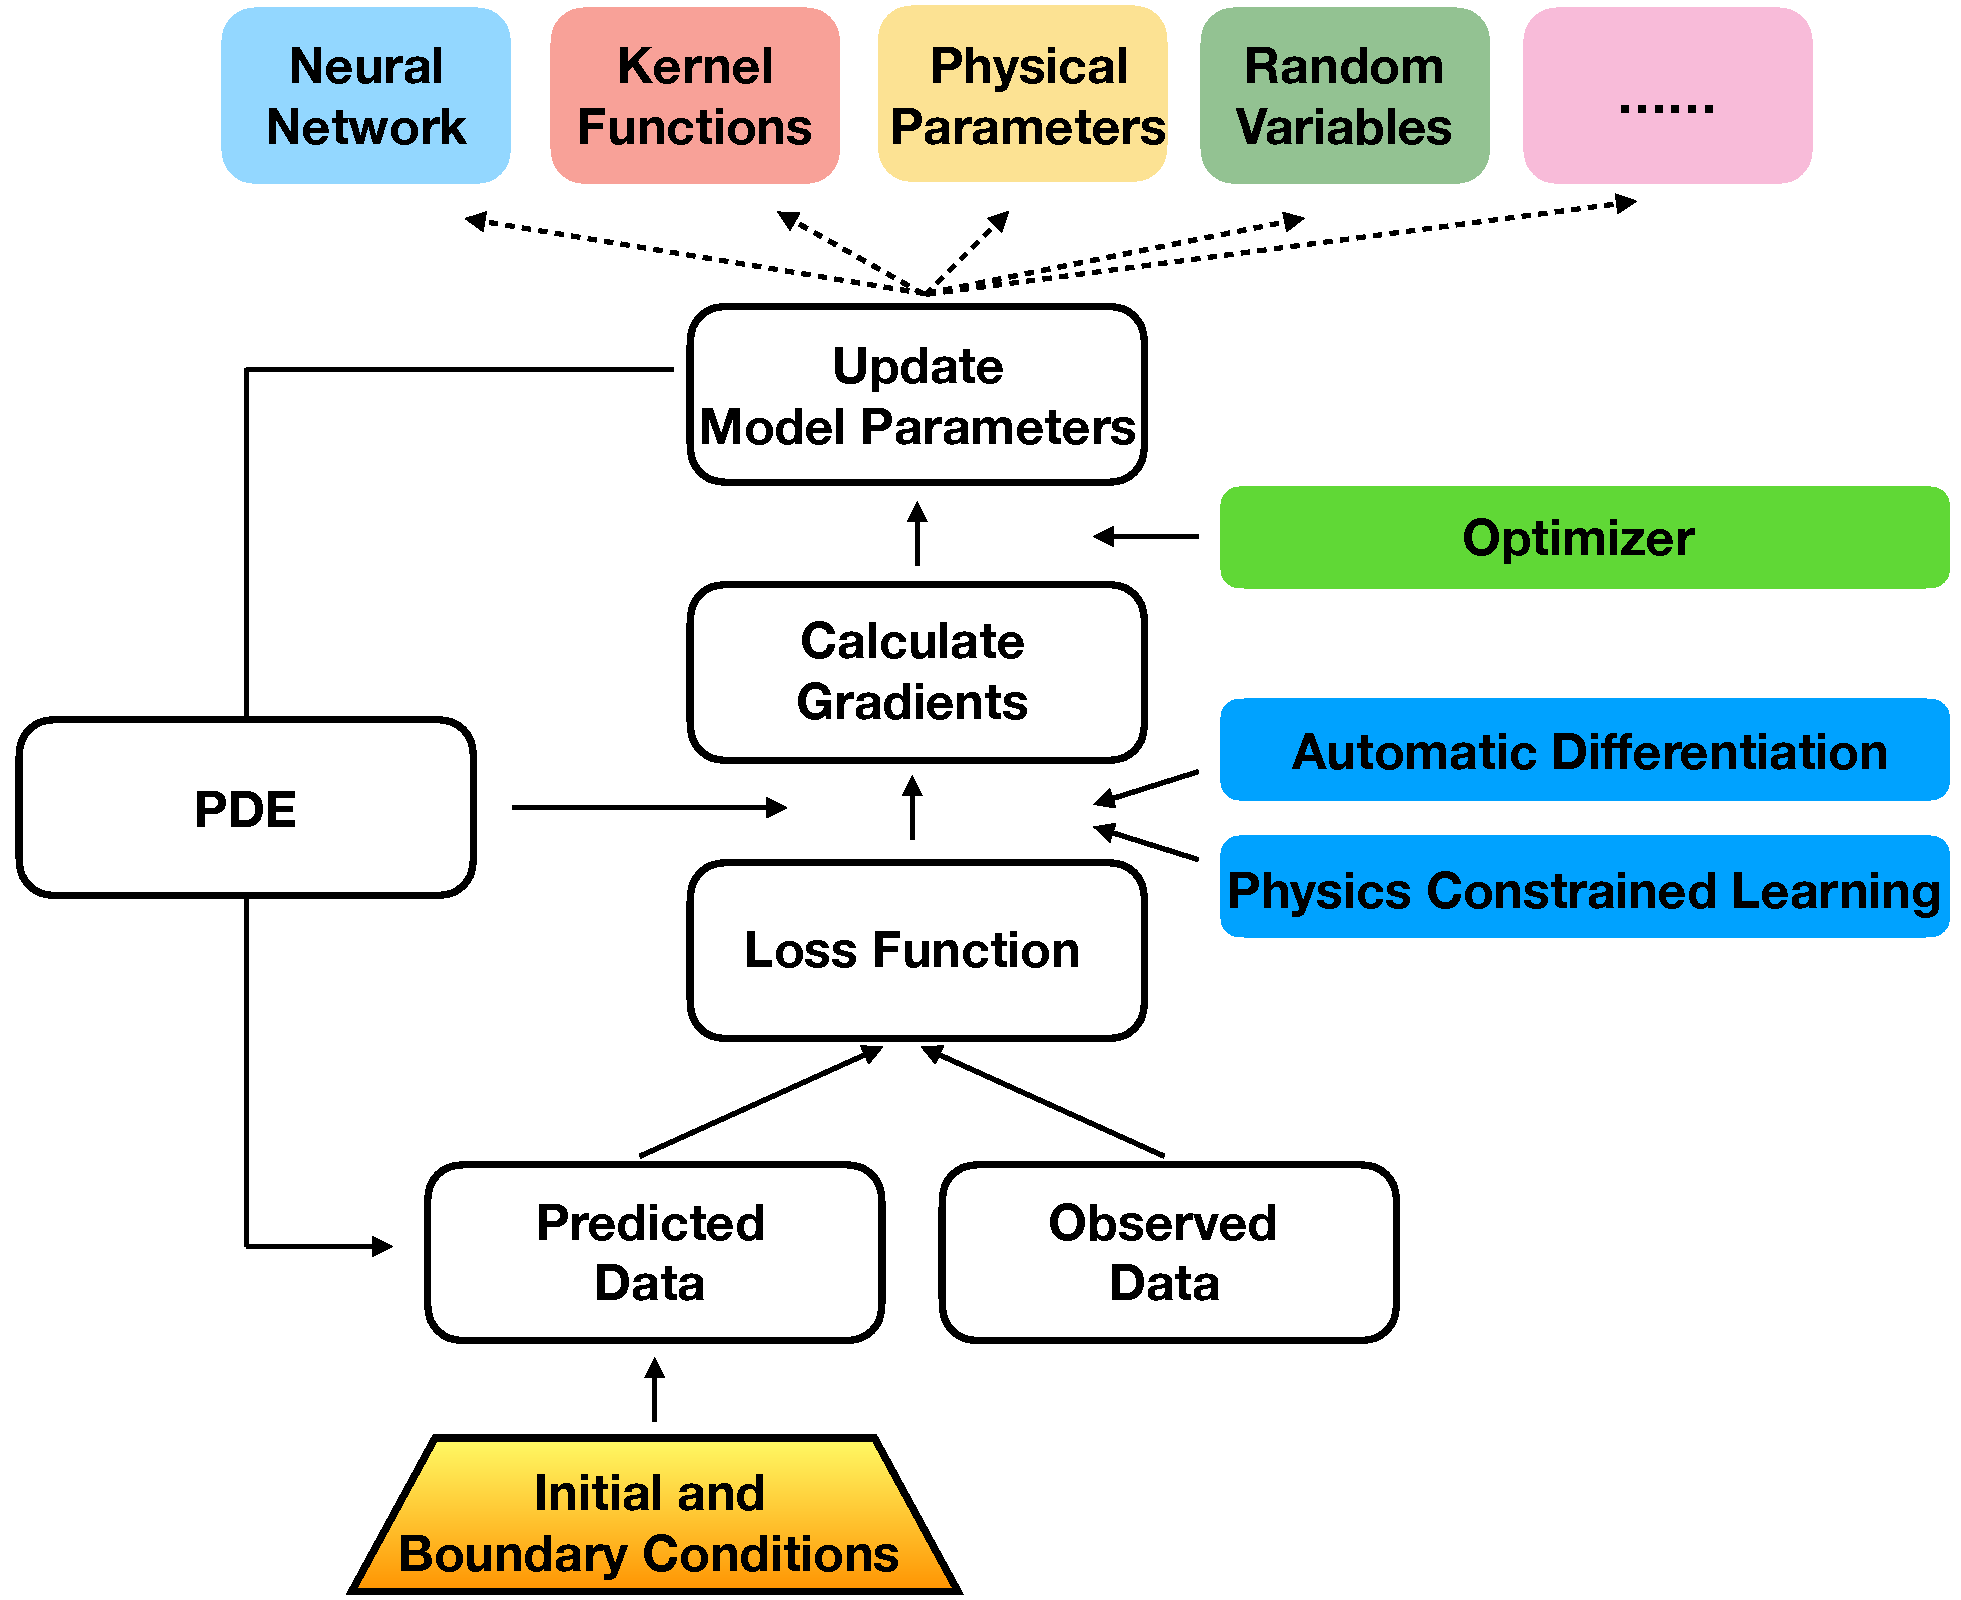
\includegraphics[width=0.8\textwidth]{figures/routine}
	\end{figure}

\end{frame}





\begin{frame}
	\frametitle{Physics Constrained Learning: Linear System}
	
	\begin{itemize}
		\item Many physical simulations require solving a linear system 
		$$A(\theta_2) u_h = \theta_1$$
		\item The corresponding PDE constraint in our formulation is  
		$$F_h(\theta_1,\theta_2, u_h) = \theta_1 - A(\theta_2)u_h = 0$$
		\item The backpropagation formula
		\begin{align*}
			p &:=\frac{\partial \tilde L_h(\theta_1, \theta_2)}{\partial \theta_1} = \frac{\partial L_h(u_h)}{\partial u_h}A(\theta_2)^{-1}\\
			q &:=\frac{\partial \tilde L_h(\theta_1, \theta_2)}{\partial \theta_2} = -\frac{\partial L_h(u_h)}{\partial u_h}A(\theta_2)^{-1} \frac{\partial A(\theta_2)}{\partial \theta_2}
		\end{align*}
		which is equivalent to 
		$$A^T p^T =\left( \frac{\partial  L_h(u_h)}{\partial u_h} \right)^T\quad q = -p\frac{\partial A(\theta_2)}{\partial \theta_2} $$
	\end{itemize}
	
\end{frame}
%\section{}
% Stochastic Inverse Problems 

\begin{frame}
	\frametitle{Methodology Summary}
\begin{figure}[hbt]
\centering
  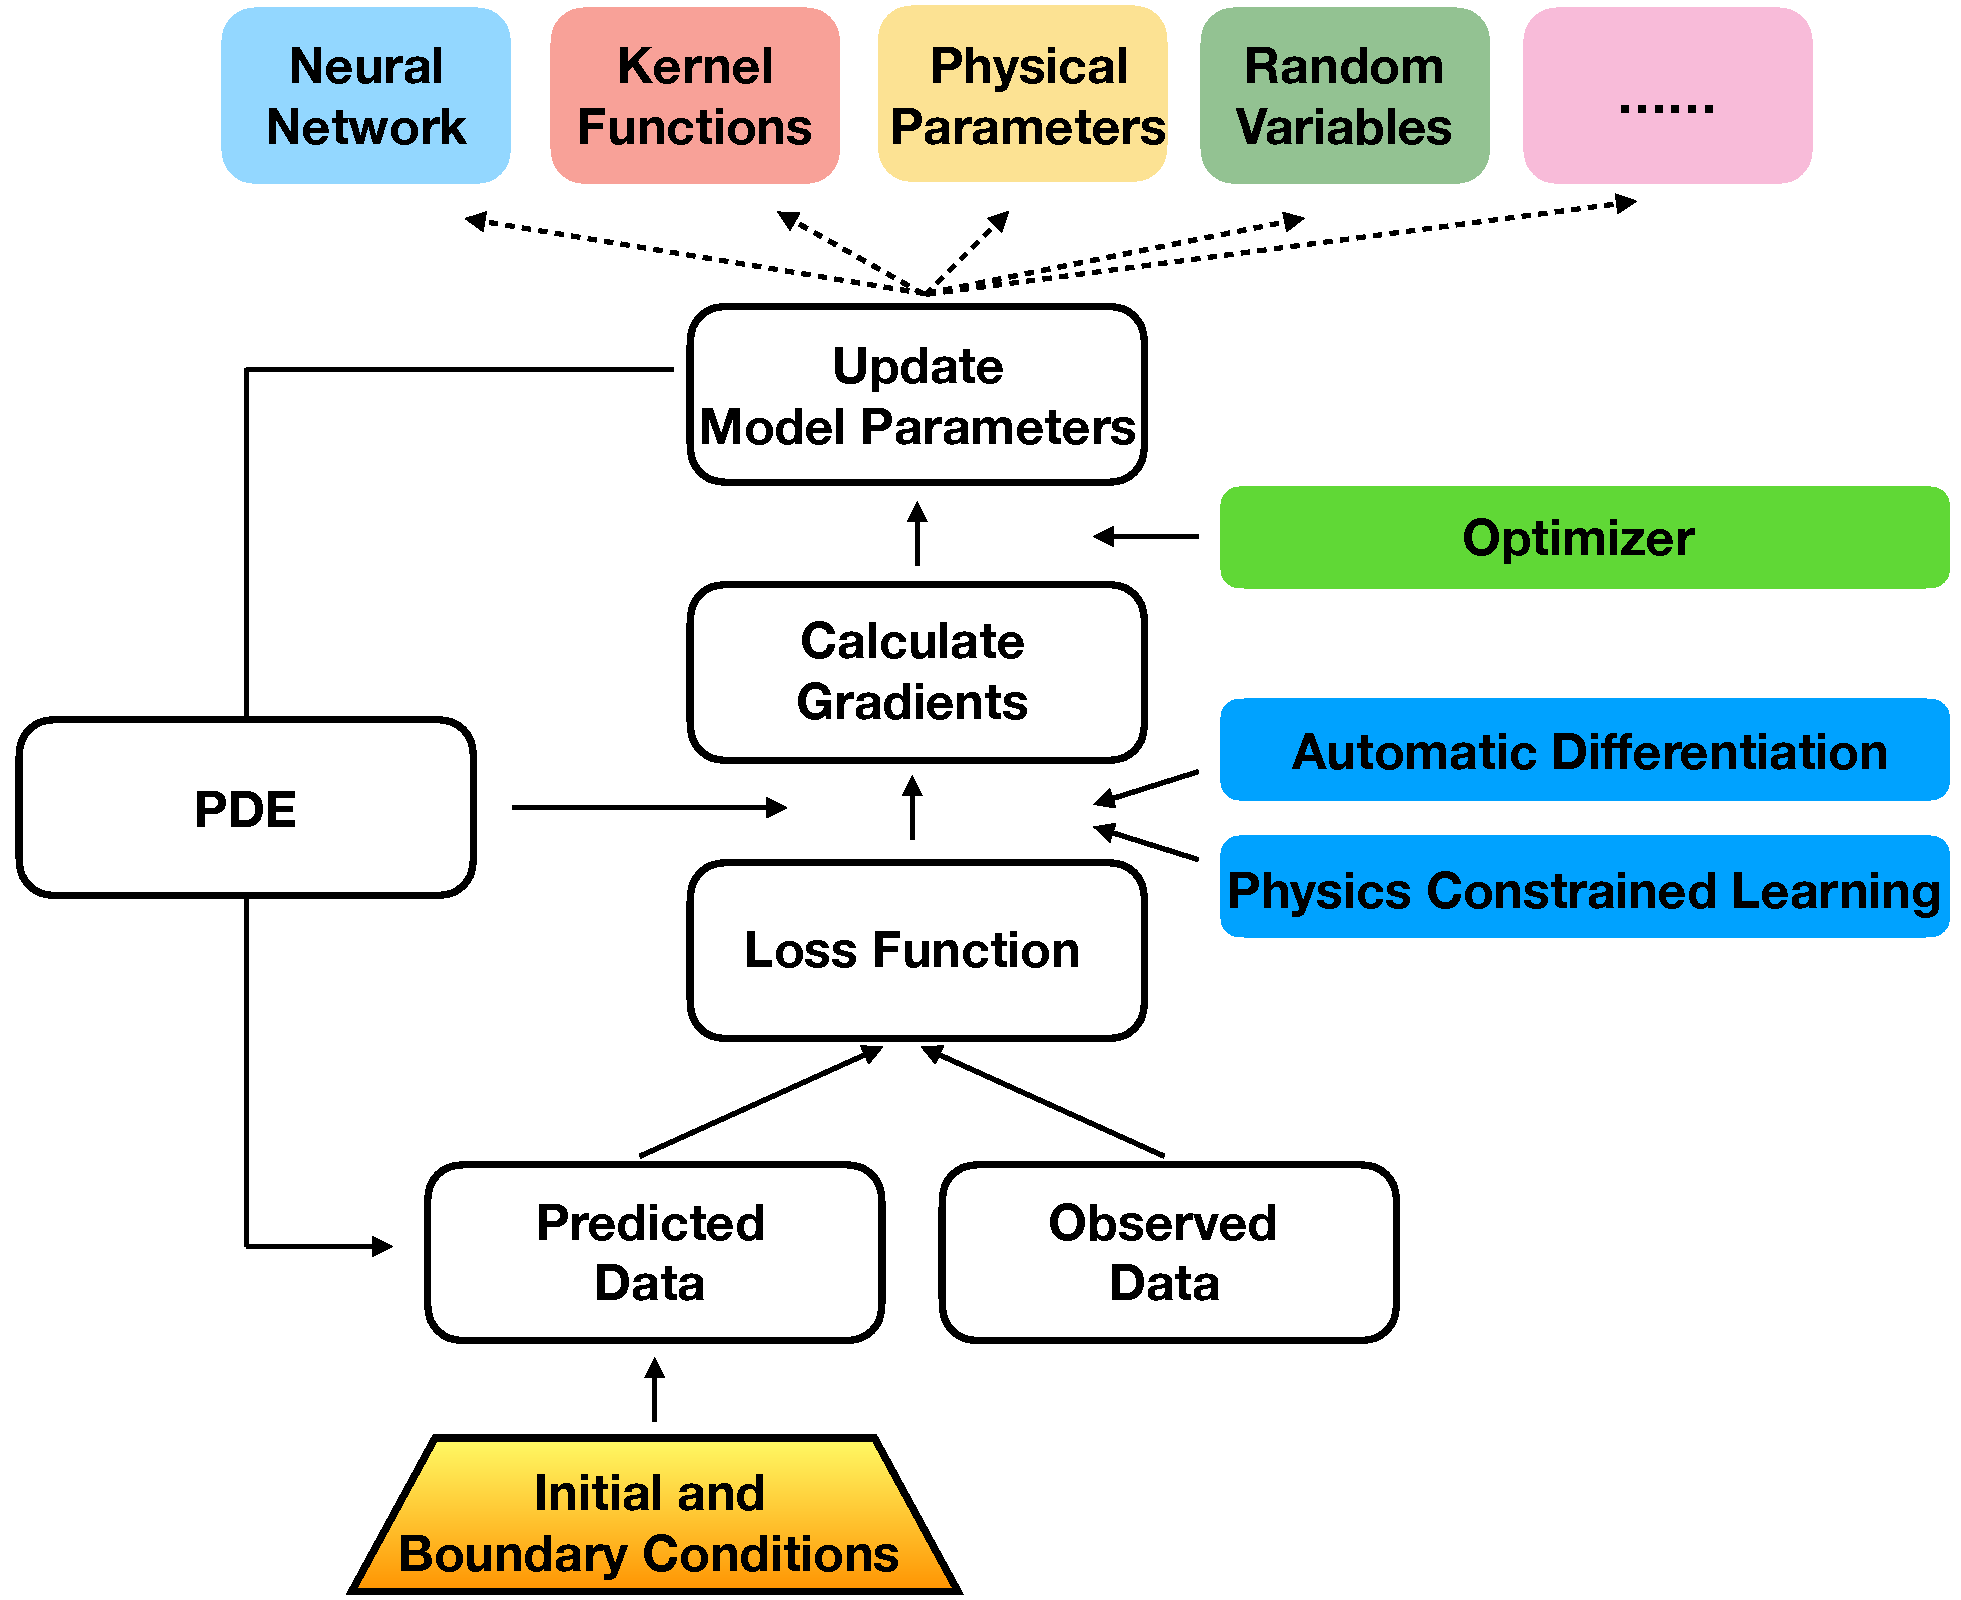
\includegraphics[width=0.8\textwidth]{figures/routine}
\end{figure}

\end{frame}


\section{Applications}


\begin{frame}
	\frametitle{ADSeismic.jl: A General Approach to Seismic Inversion}
	\begin{itemize}
		\item Many seismic inversion problems can be solved within a unified framework. 
	\end{itemize}
	\begin{figure}[hbt]
  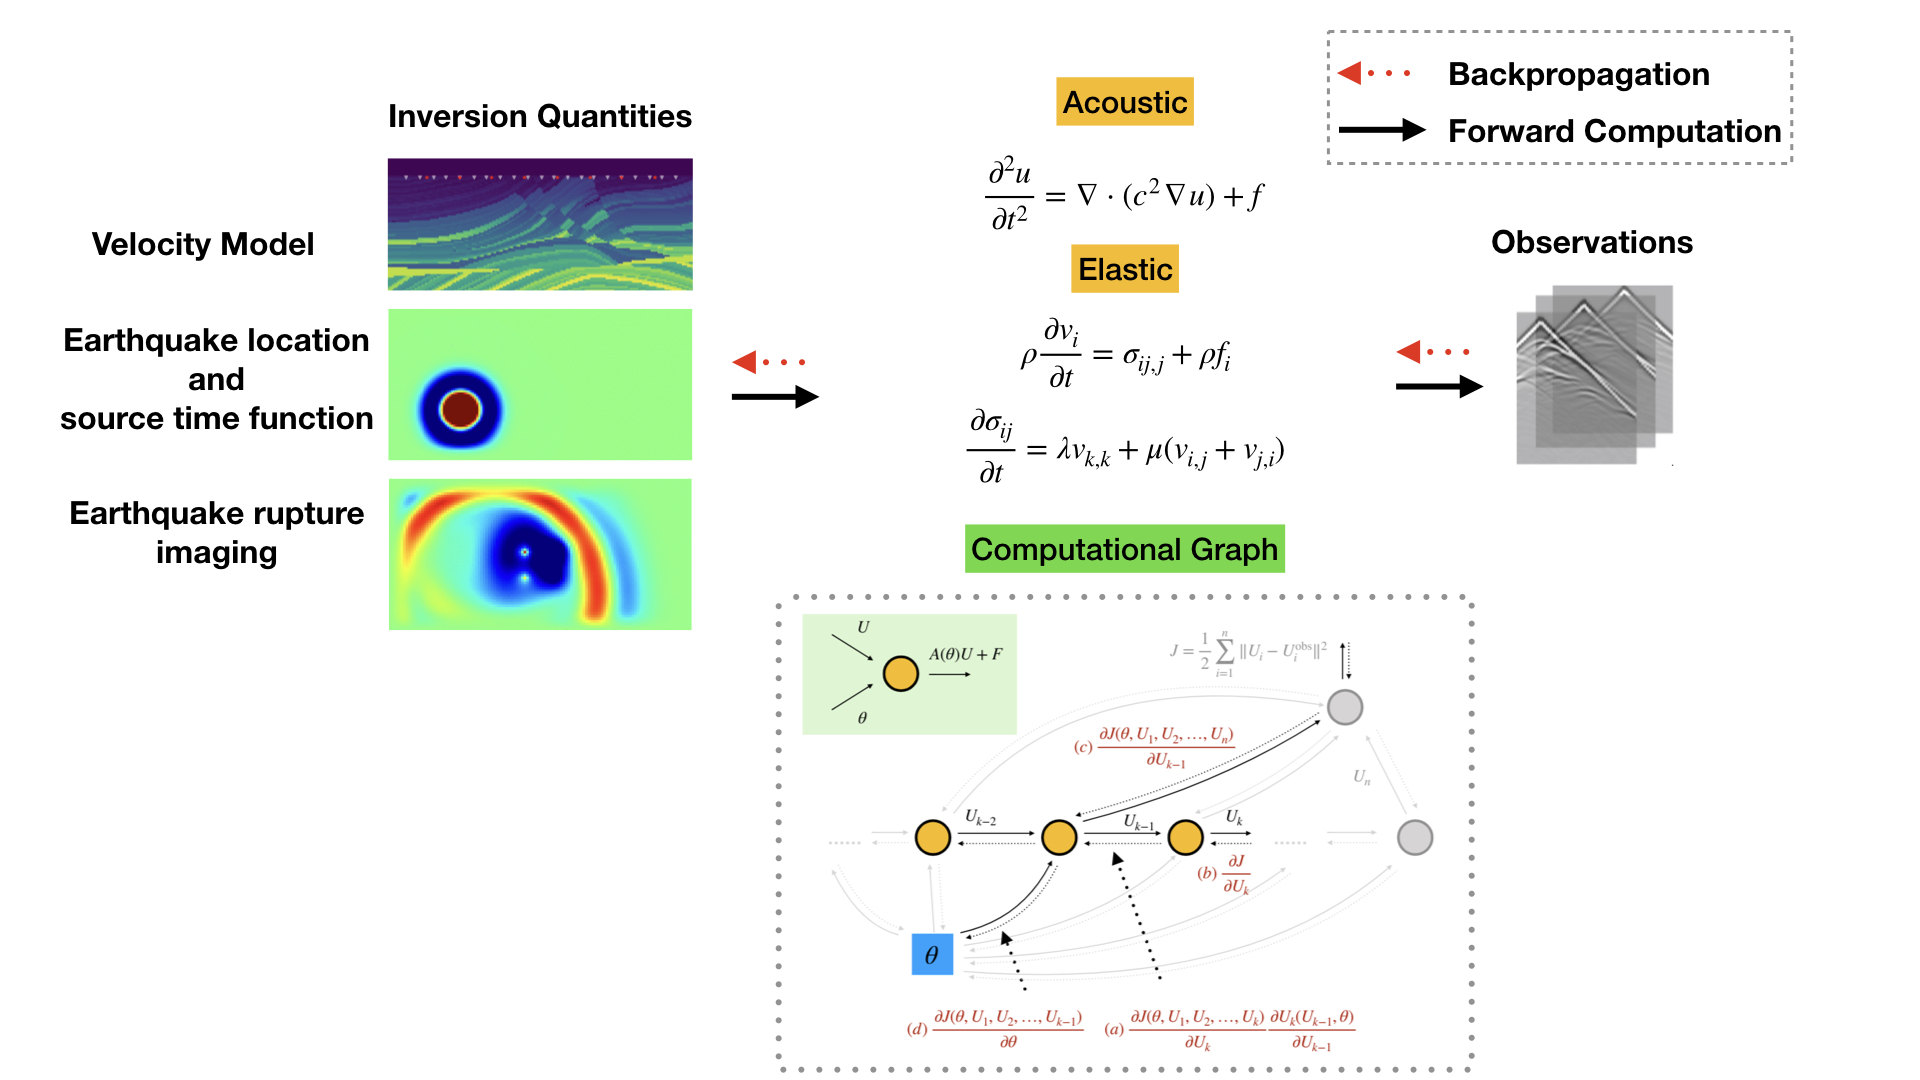
\includegraphics[width=1.0\textwidth]{figures/adseimic.jpeg}
\end{figure}
	
\end{frame}

\begin{frame}
	\frametitle{ADSeismic.jl: Earthquake Location Example}
	\begin{itemize}
		\item The earthquake source function is parameterized by ($g(t)$ and $x_0$ are unknowns)
		$$f(x, t) =  \frac{g(t)}{2\pi \sigma^2} \exp \left( -\frac{||x - x_0||^2}{2 \sigma^2} \right)$$
	\end{itemize}
	\begin{figure}[hbt]
  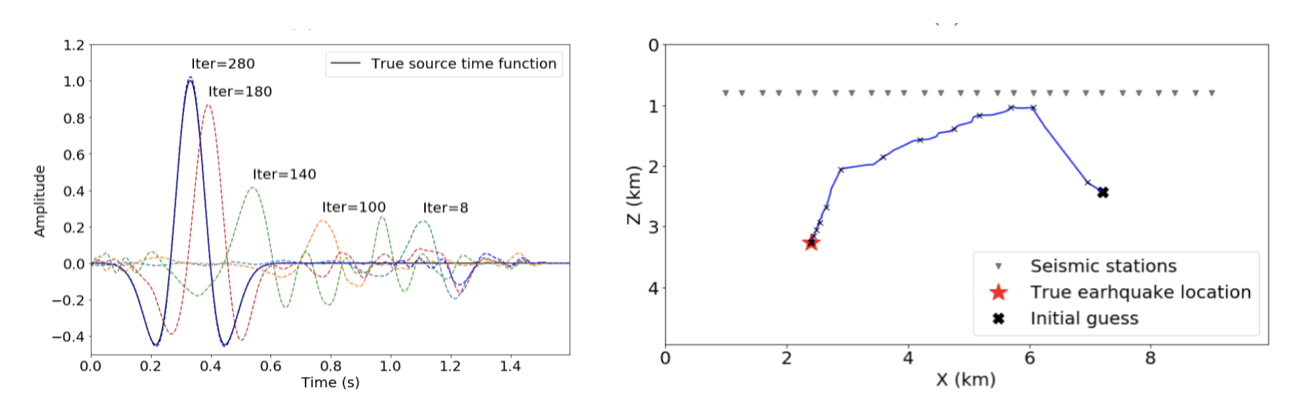
\includegraphics[width=1.0\textwidth]{figures/source_time}
\end{figure}
\end{frame}


\begin{frame}
	\frametitle{ADSeismic.jl: Benchmark}
	\begin{itemize}
		\item ADCME makes the heterogeneous computation capability of TensorFlow available for scientific computing. 
	\end{itemize}
	\begin{figure}[hbt]
  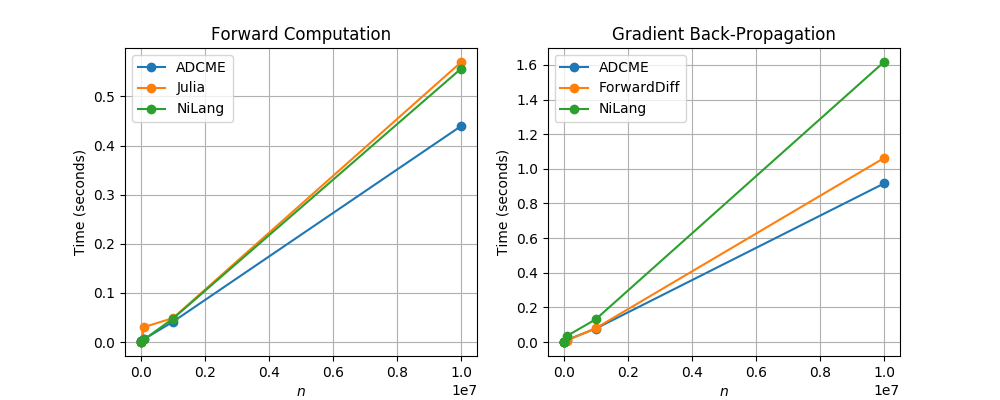
\includegraphics[width=0.7\textwidth]{figures/benchmark}
\end{figure}
\end{frame}

\begin{frame}
	\frametitle{NNFEM.jl: Constitutive Modeling}
	
	\begin{equation}\label{equ:momentum}
  \begin{aligned}
		\underbrace{\sigma_{ij,j}}_{\mbox{stress}} + \rho \underbrace{b_i}_{\mbox{external force}} &= \rho \underbrace{\ddot u_i}_{\mbox{velocity}}\\
		\underbrace{\varepsilon_{ij}}_{\mbox{strain}} &= \frac{1}{2}(u_{j,i}+u_{i,j})
	\end{aligned}
\end{equation}

	
	\begin{itemize}
		\item \textbf{Observable}: external/body force $b_i$, displacements $u_i$ (strains $\varepsilon_{ij}$ can be computed from $u_i$); density $\rho$ is known.  
		\item \textbf{Unobservable}: stress $\sigma_{ij}$. 
		\item Data-driven Constitutive Relations: modeling the strain-stress relation using a neural network
\begin{equation}\label{equ:nn}
  	\boxed{\mbox{stress} =\mathcal{M}_{\theta}(\mbox{strain},\ldots)}
\end{equation}
		and the neural network is trained by coupling (1) and (2).
	\end{itemize}


\end{frame}

\begin{frame}
	\frametitle{NNFEM.jl: Robustic Constitutive Modeling}
	\begin{itemize}
\item Proper form of constitutive relation is crucial for numerical stability
{\footnotesize\begin{align*}
 \mbox{Elasticity} &\Rightarrow \bm\sigma = \mathsf{C}_{\theta}\bm\epsilon \\
\mbox{Hyperelasticity } &\Rightarrow \begin{cases}\bm\sigma =\mathcal{M}_{\theta}(\bm\epsilon) & \mbox{(Static)} \\
\bm{\sigma}^{n+1}  =  \ChoL_{\bt}(\bm\epsilon^{n+1}) \ChoL_{\bt}(\bm\epsilon^{n+1})^T (\bm{\epsilon}^{n+1} - \bm{\epsilon}^{n})  + \bm{\sigma}^{n}  & \mbox{(Dynamic)} \end{cases} \\
	\mbox{Elaso-Plasticity} &\Rightarrow \bm\sigma^{n+1} = \ChoL_{\bt}(\bm\epsilon^{n+1},\bm{\epsilon}^{n},\bm{\sigma}^{n}) \ChoL_{\bt}(\bm\epsilon^{n+1},\bm{\epsilon}^{n},\bm{\sigma}^{n})^T (\bm{\epsilon}^{n+1} - \bm{\epsilon}^{n})  + \bm{\sigma}^{n} 
\end{align*}
}{\footnotesize$$\ChoL_{\bt} = \begin{bmatrix}
L_{1111}  &  & &  &       &\\
L_{2211}  & L_{2222} & &   & &\\
 L_{3311}  &  L_{3322}               & L_{3333} &  & &\\
               &                 &                 & L_{2323}&  &\\
              &               &                  &                & L_{1313} &\\
              &                 &                  &                &                 &L_{1212}\\
\end{bmatrix}$$}
	\item \textcolor{red}{Weak convexity}: $\ChoL_{\bt}\ChoL_{\bt}^T \succ 0$
	\item \textcolor{red}{Time consistency}:  $\bm\sigma^{n+1} \rightarrow \bm \sigma^n$ when $\bm\epsilon^{n+1} \rightarrow \bm \epsilon^n$
\end{itemize}

\end{frame}

\begin{frame}
	\frametitle{NNFEM.jl: Robustic Constitutive Modeling}
	\begin{itemize}
	 \item Weak form of balance equations of linear momentum 
	{\footnotesize
	\begin{align*}
		P_i(\theta) &= \int_V \rho \ddot u_i \delta u_i dVt + \int_{V} \textcolor{blue}{\underbrace{\textcolor{blue}{\sigma_{ij}(\theta)}}_{\mathclap{\textcolor{blue}{\mbox{embedded neural network}}}}} \delta \varepsilon_{ij}dV\\
		F_i &= \int_{V}\rho b_i \delta u_i dV + \int_{\partial V} t_i\delta u_idS
	\end{align*}
	}
	\item Train the neural network by 
	{\scriptsize $$\boxed{L(\theta) = \min_{\theta}\;\sum_{i=1}^N(P_i(\theta) - F_i)^2}$$}
	The gradient $\nabla L(\theta)$ is computed via automatic differentiation.
	\end{itemize}
	\begin{figure}[hbt]
  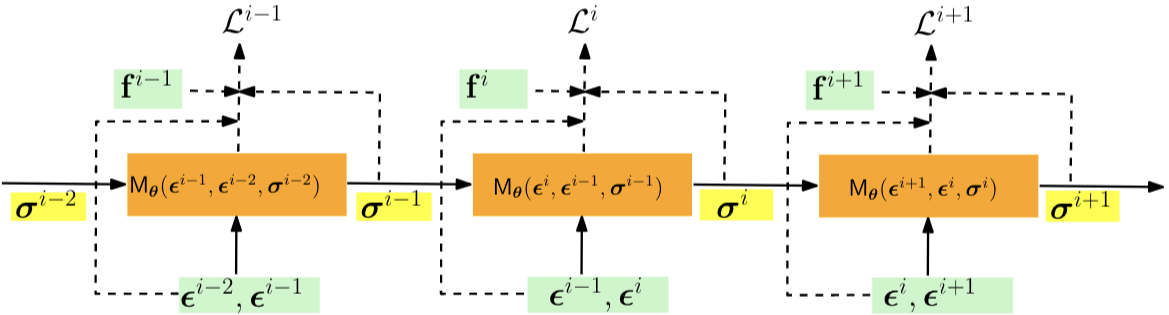
\includegraphics[width=0.75\textwidth]{figures/rnn}
\end{figure}

\end{frame}

\begin{frame}
	\frametitle{NNFEM.jl: Robustic Constitutive Modeling}
\begin{figure}[hbt]
  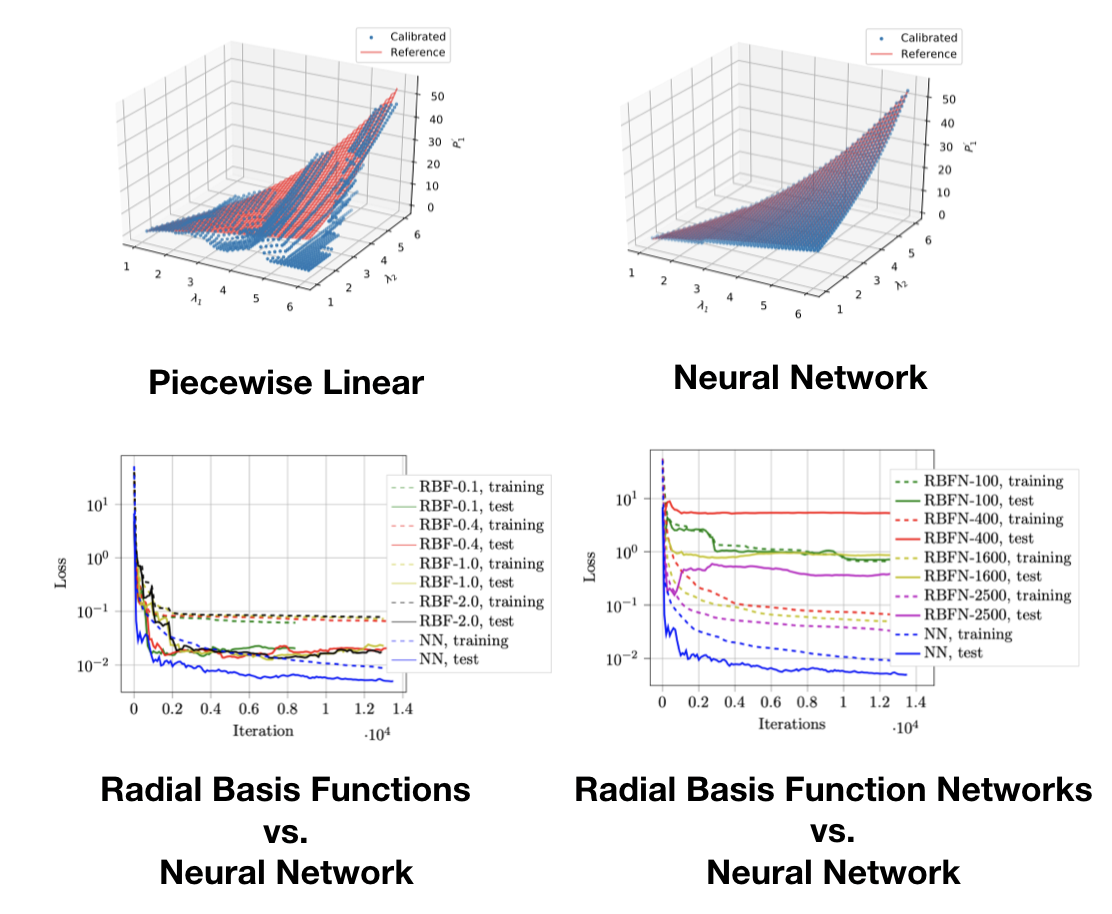
\includegraphics[width=0.8\textwidth]{figures/vs}
\end{figure}
\end{frame}


\begin{frame}
	\frametitle{NNFEM.jl: Robustic Constitutive Modeling}
	\begin{itemize}
		\item Comparison of different neural network architectures 
		\begin{align*}
			\bm\sigma^{n+1} &= \ChoL_{\bt}(\bm\epsilon^{n+1},\bm{\epsilon}^{n},\bm{\sigma}^{n}) \ChoL_{\bt}(\bm\epsilon^{n+1},\bm{\epsilon}^{n},\bm{\sigma}^{n})^T (\bm{\epsilon}^{n+1} - \bm{\epsilon}^{n})  + \bm{\sigma}^{n} \\
			\bm{\sigma}^{n+1} &=  \mathsf{NN}_{\bt}(\bm\epsilon^{n+1},\bm{\epsilon}^{n},\bm{\sigma}^{n})\\
			\bm{\sigma}^{n+1} &=  \mathsf{NN}_{\bt}(\bm\epsilon^{n+1},\bm{\epsilon}^{n},\bm{\sigma}^{n}) + \bm{\sigma}^{n}
		\end{align*}
	\end{itemize}
\begin{figure}[hbt]
  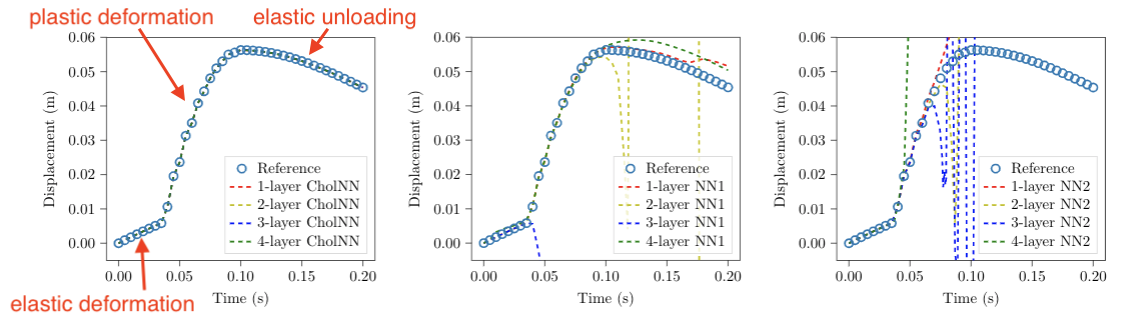
\includegraphics[width=1.0\textwidth]{figures/nncons}
\end{figure}
\end{frame}




\begin{frame}
	\frametitle{FwiFlow.jl: Elastic Full Waveform Inversion for subsurface flow problems}
	\begin{figure}[hbt]
  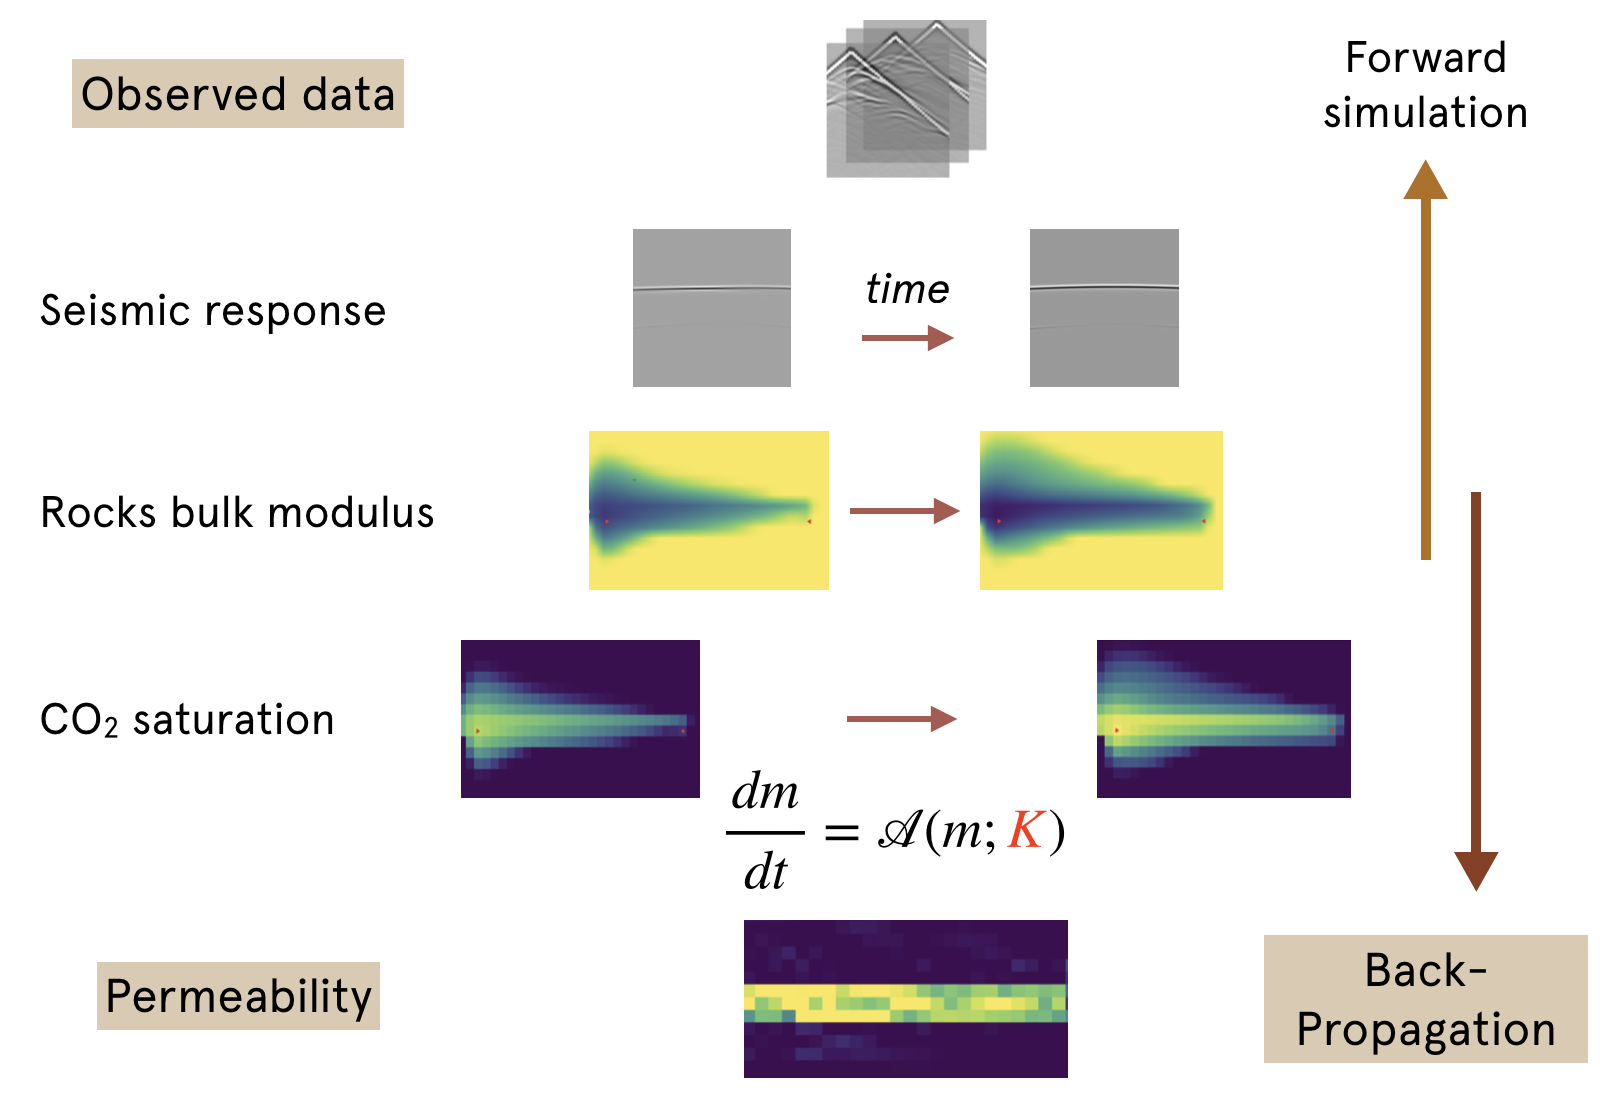
\includegraphics[width=0.8\textwidth]{figures/geo.png}
\end{figure}
\end{frame}

\begin{frame}
\frametitle{FwiFlow.jl: Fully Nonlinear Implicit Schemes}
\begin{itemize}
	\item The governing equation is a nonlinear PDE
{\scriptsize
	\begin{align*}
	\frac{\partial }{{\partial t}}(\phi {{S_i}}{\rho _i}) + \nabla  \cdot ({\rho _i}{\mathbf{v}_i}) &= {\rho _i}{q_i},\quad 
      i = 1,2	\\
      S_{1} + S_{2} &= 1\\
      {\mathbf{v}_i} &= - \frac{{\textcolor{blue}{K}{\textcolor{red}{k_{ri}}}}}{{{\tilde{\mu}_i}}}(\nabla {P_i} - g{\rho _i}\nabla Z), \quad
      i=1, 2\\
	k_{r1}(S_1) =& \frac{k_{r1}^o S_1^{L_1}}{S_1^{L_1} + E_1 S_2^{T_1}}\\
	k_{r2}(S_1) =& \frac{ S_2^{L_2}}{S_2^{L_2} + E_2 S_1^{T_2}}
	\end{align*}
	}
	\item For stability and efficiency, implicit methods are the industrial standards. 
{\scriptsize	$$\phi (S_2^{n + 1} - S_2^n) - \nabla \cdot \left( {{m_{2}}(S_2^{n + 1})K\nabla \Psi _2^n} \right) \Delta t = 
\left(q_2^n + q_1^n \frac{m_2(S^{n+1}_2)}{m_1(S^{n+1}_2)}\right) 
\Delta t\quad m_i(s) = \frac{k_{ri}(s)}{\tilde \mu_i}
$$}
\item It is impossible to express the numerical scheme directly in an AD framework. Physics constrained learning is used to enhance the AD framework for computing gradients. 
\end{itemize}

\end{frame}

\begin{frame}
	\frametitle{FwiFlow.jl: Showcase}
	\begin{itemize}
		\item Task 1: Estimating the permeability from seismic data 
		\begin{center}
	B.C. +	\textcolor{red}{Two-Phase Flow Equation} + Wave Equation $\Rightarrow$ Seismic Data
	\end{center}
		\begin{figure}[hbt]
		\centering
  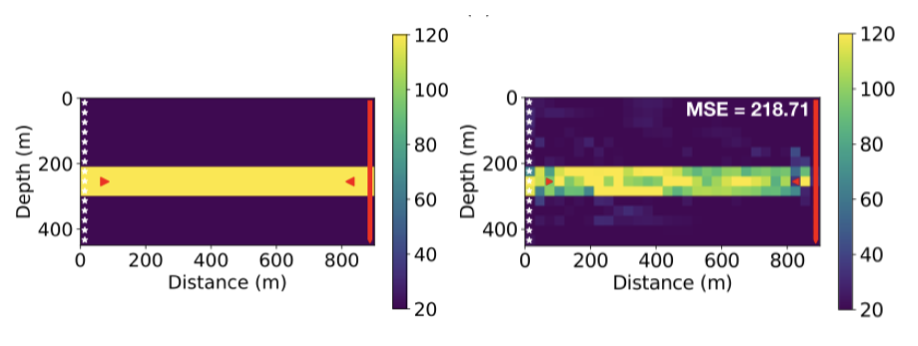
\includegraphics[width=0.6\textwidth]{figures/coupled}
\end{figure}
\item Task 2: Learning the rock physics model from sparse saturation data. The rock physics model is approximated by neural networks  
{\scriptsize$$f_1(S_1; \theta_1) \approx k_{r1}(S_1)\qquad f_2(S_1; \theta_2) \approx k_{r2}(S_1)$$}
\vspace{-0.4cm}
\begin{figure}
	\centering
	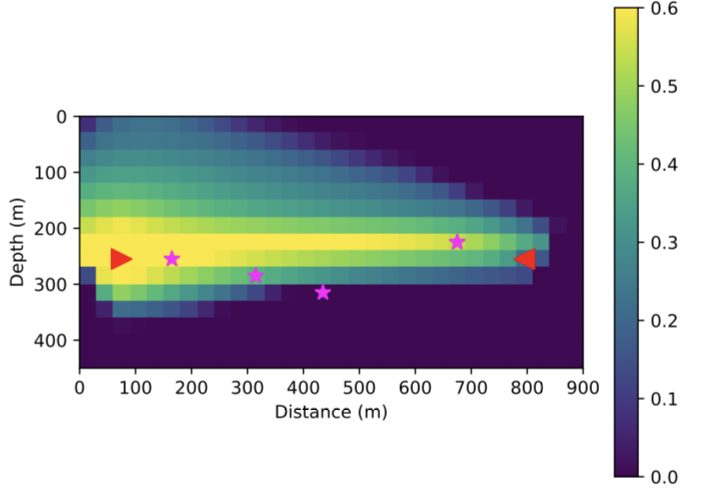
\includegraphics[width=0.3\textwidth]{figures/sat}~
  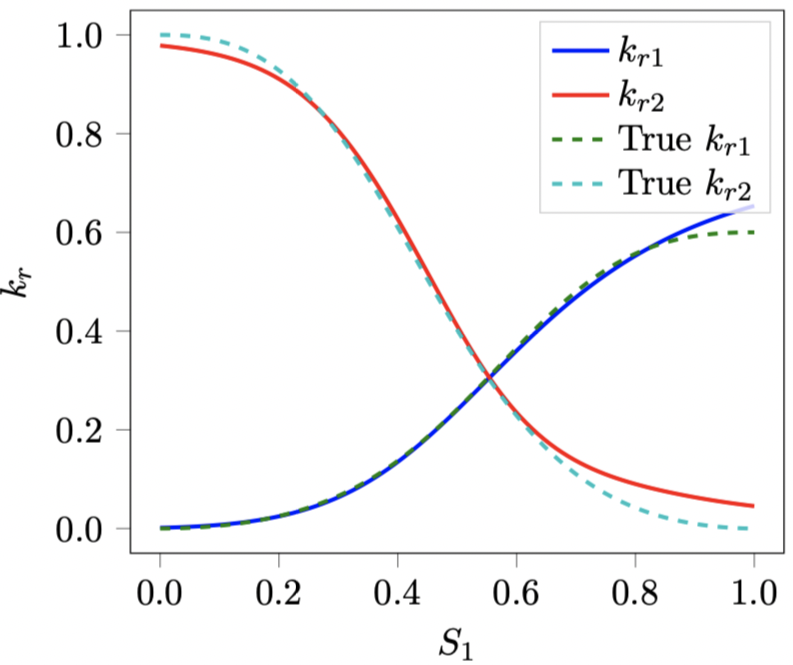
\includegraphics[width=0.25\textwidth]{figures/rock}
\end{figure}
	\end{itemize}
\end{frame}

\begin{frame}
	\frametitle{FwiFlow.jl: Showcase}
	\begin{itemize}
		\item Task 3: Learning the \textcolor{red}{nonlocal} (space or time) hidden dynamics from seismic data. This is very challenging using traditional methods (e.g., the adjoint-state method) because the dynamics is history dependent. 
	\end{itemize}
	\begin{center}
	B.C. +	\textcolor{red}{Time-/Space-fractional PDE} + Wave Equation $\Rightarrow$ Seismic Data
	\end{center}
\begin{table}[htpb]
\centering
\begin{tabular}{@{}lll@{}}
\toprule
Governing Equation & $\sigma=0$ & $\sigma=5$ \\ \midrule
${}_0^CD_t^{\textbf{0.8}}m = 10\Delta m $ & \makecell{$a/a^*\ =1.0000$ \\  $\quad\alpha\quad =\mathbf{0.8000}$} & \makecell{$a/a^*\ =0.9109$ \\  $\quad\alpha\quad =\mathbf{0.7993}$} \\ \hline
${}_0^CD_t^{\textbf{0.2}}m = 10\Delta m $ & \makecell{$a/a^*\ =0.9994$ \\  $\quad\alpha\quad =\mathbf{0.2000}$} & \makecell{$a/a^*\ =0.3474$ \\  $\quad\alpha\quad =\mathbf{0.1826}$}  \\   \bottomrule
$\frac{\partial m}{\partial t} = -10(-\Delta)^{\textbf{0.2}} m$ & \makecell{$a/a^*\ =1.0000$ \\   $\quad s\quad =\mathbf{0.2000}$} & \makecell{$a/a^*\ =1.0378$ \\   $\quad s\quad =\mathbf{0.2069}$} \\  \hline
$\frac{\partial m}{\partial t} = -10(-\Delta)^{\textbf{0.8}} m$ & \makecell{$a/a^*\ =1.0000$ \\   $\quad s\quad =\mathbf{0.8000}$} & \makecell{$a/a^*\ =1.0365$ \\   $\quad s\quad =\mathbf{0.8093}$}\\  \bottomrule
\end{tabular}
\end{table}

\end{frame}


\newcommand{\bsigma}[0]{\bm{\sigma}}
\newcommand{\bepsilon}[0]{\bm{\epsilon}}


\begin{frame}
	\frametitle{PoreFlow.jl: Inverse Modeling of Viscoelasticity}
%	
	\begin{itemize}
		\item Multi-physics Interaction of Coupled Geomechanics and Multi-Phase Flow Equations 
{\small
\begin{align*}
\mathrm{div}\bsigma(\bu) - b \nabla p &= 0\\
    \frac{1}{M} \frac{\partial p}{\partial t} + b\frac{\partial \epsilon_v(\bu)}{\partial t} - \nabla\cdot\left(\frac{k}{B_f\mu}\nabla p\right) &= f(x,t)	\\
    	\bsigma &= \bsigma(\bepsilon, \dot\bepsilon)
\end{align*}
}
\item Approximate the constitutive relation by a neural network
{\small
 $$\bsigma^{n+1} - \bsigma^{n} = \mathcal{NN}_{\bt} (\bsigma^n, \bepsilon^n) + H (\bepsilon^{n+1} - \bepsilon^n)$$}
	\end{itemize}		
	\begin{figure}[hbt]	
	\centering
  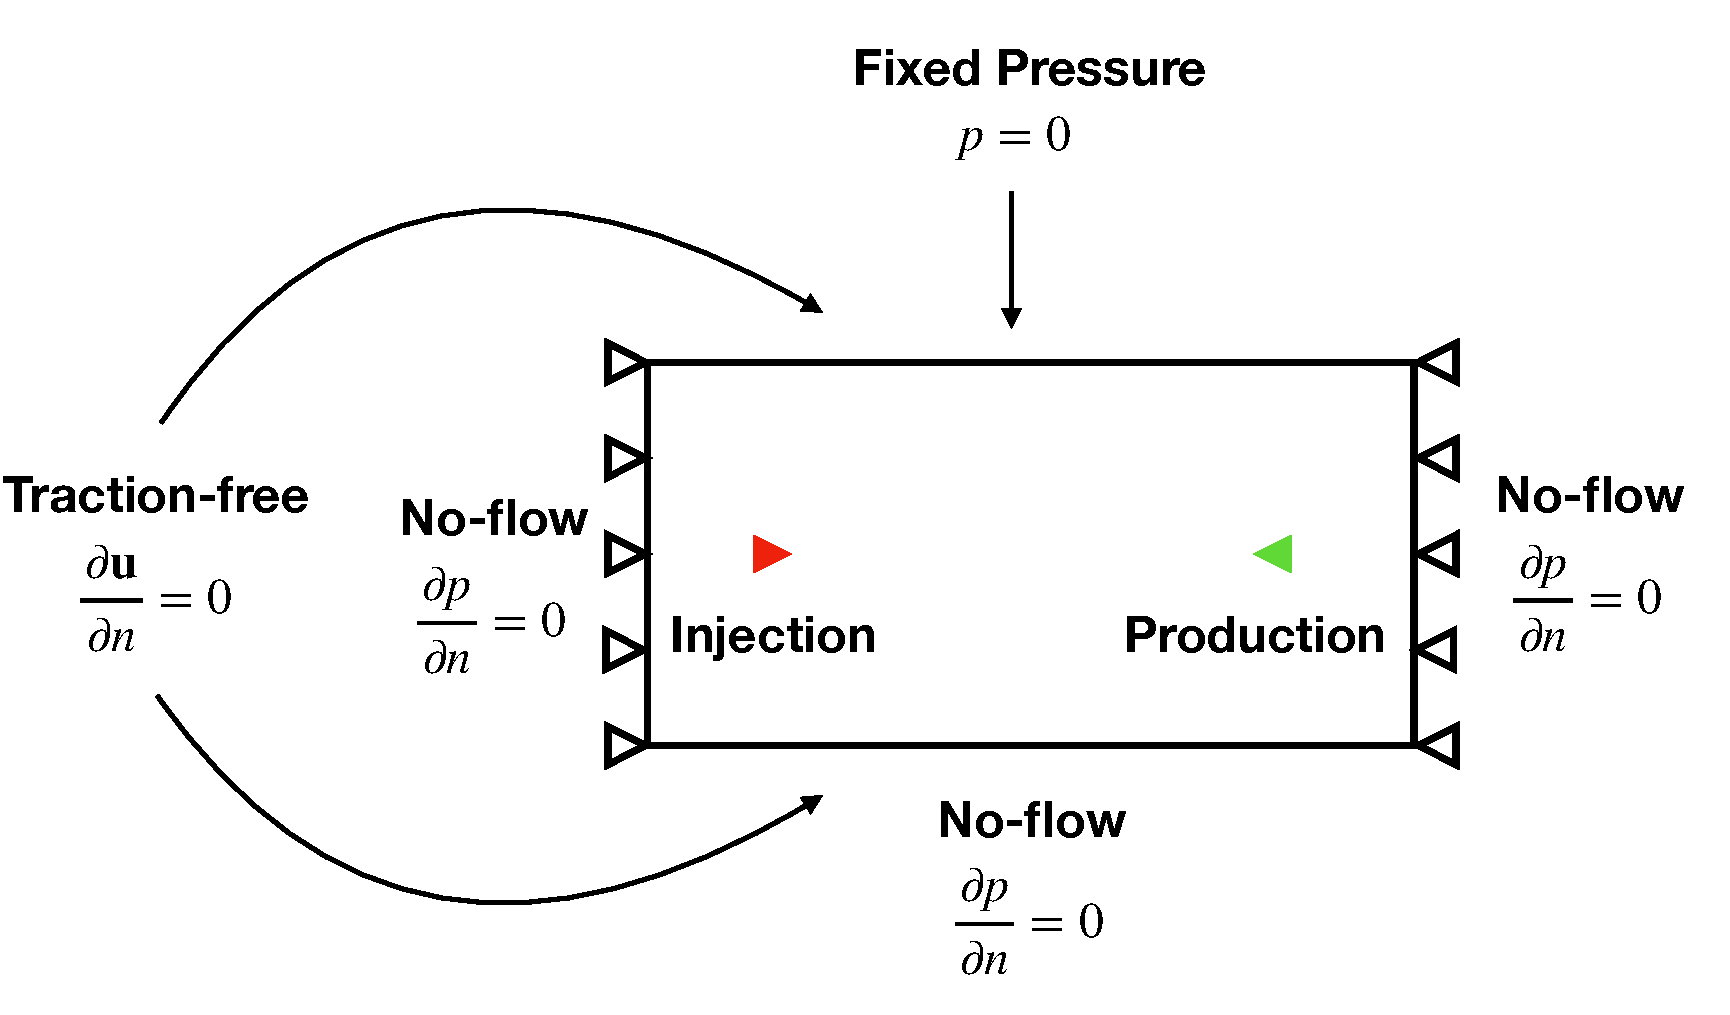
\includegraphics[width=0.5\textwidth]{figures/ip}~
  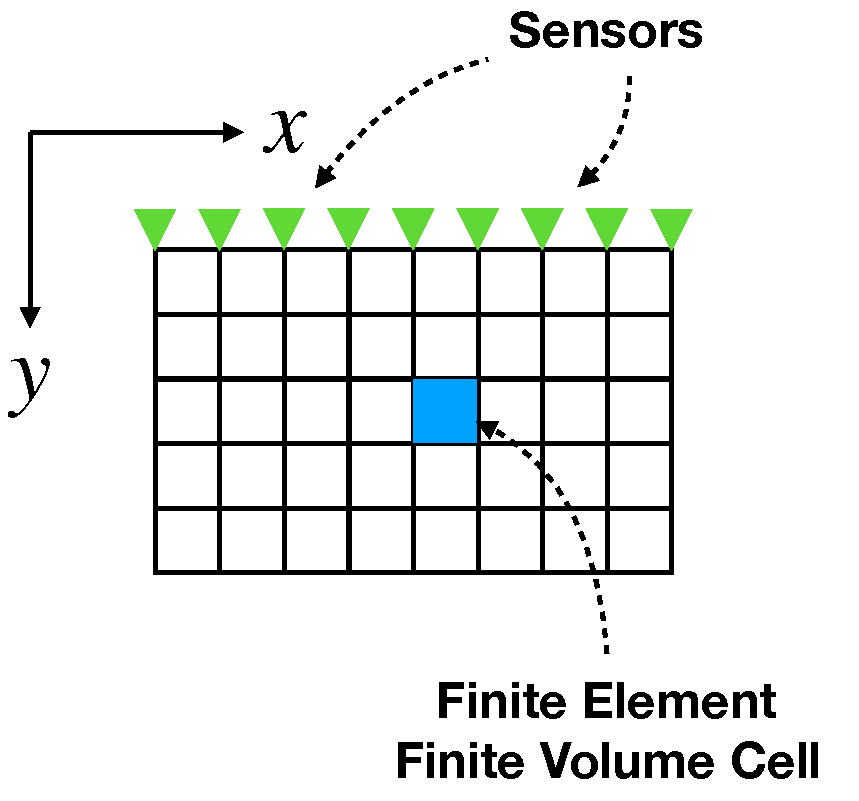
\includegraphics[width=0.3\textwidth]{figures/cell}
\end{figure}

\end{frame}


\begin{frame}
	\frametitle{PoreFlow.jl: Inverse Modeling of Viscoelasticity}
	
	\begin{itemize}
		\item Comparison with space varying linear elasticity approximation
		\begin{equation}
			\bsigma = H(x, y) \bepsilon
		\end{equation}
	\end{itemize}
	\begin{figure}[hbt]
  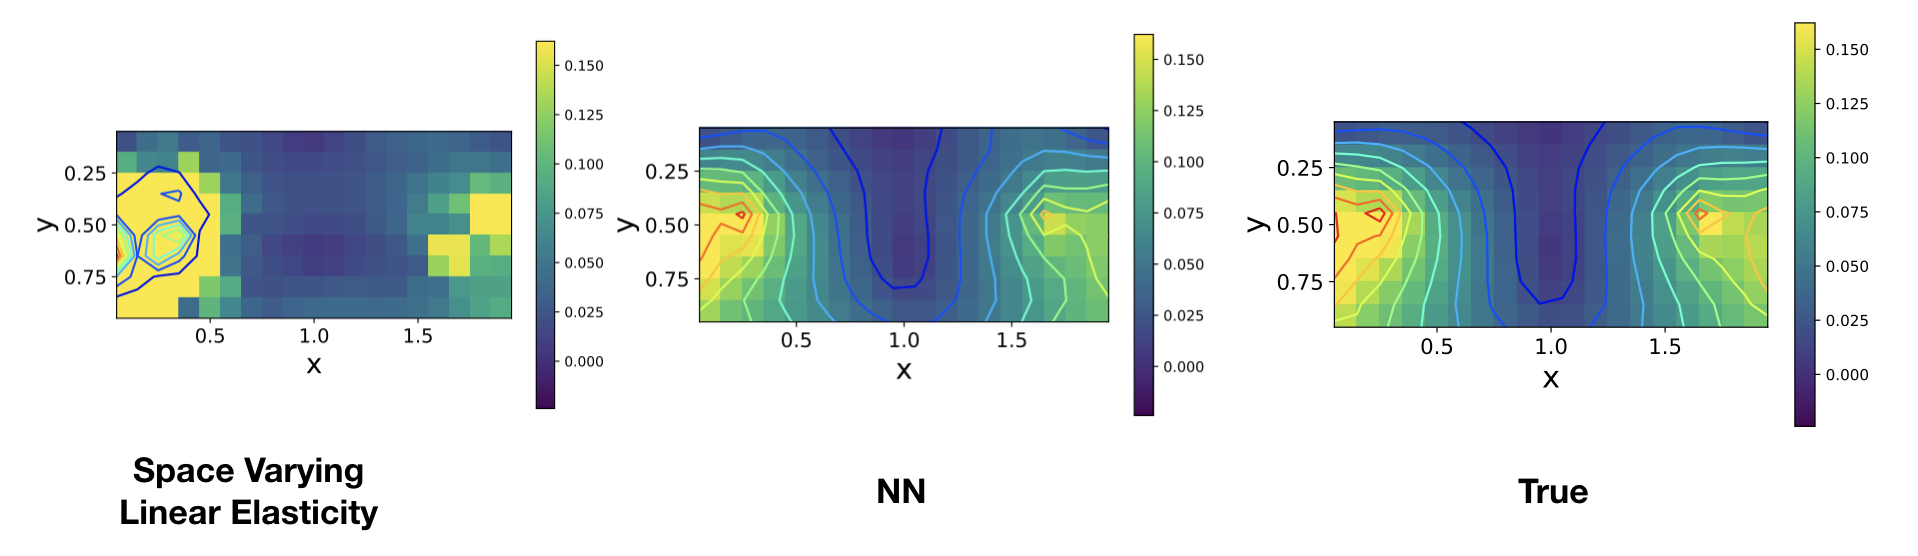
\includegraphics[width=1.0\textwidth]{figures/visco1}
\end{figure}

\end{frame}

\begin{frame}
	\frametitle{PoreFlow.jl: Inverse Modeling of Viscoelasticity}
	\begin{figure}[hbt]
  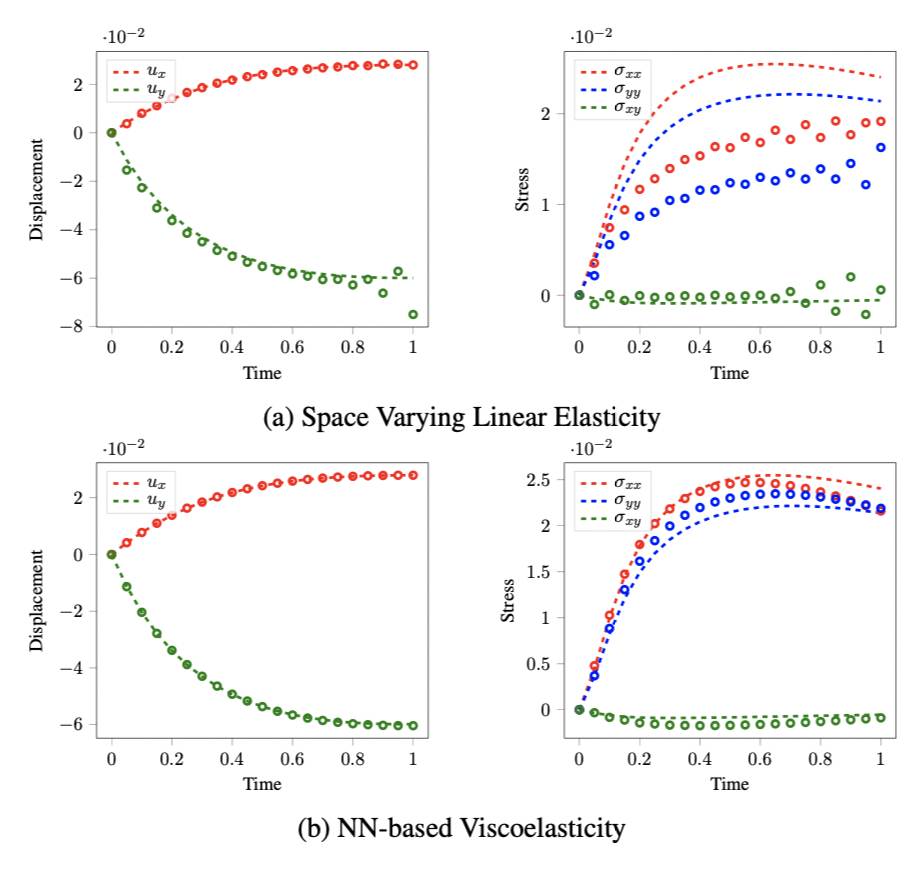
\includegraphics[width=0.7\textwidth]{figures/visco2}
\end{figure}

\end{frame}



\section{Some Perspectives}

\begin{frame}
	\frametitle{A Parameter/Function Learning View of Inverse Modeling}
	% Please add the following required packages to your document preamble:
% \usepackage{booktabs}
\begin{itemize}
	\item Most inverse modeling problems can be classified into 4 categories. To be more concrete, consider the PDE for describing physics
	\begin{equation}
		\nabla \cdot (\textcolor{red}{\theta} \nabla u(x)) = 0\quad \mathcal{B}\mathcal{C}(u(x)) = 0
	\end{equation}
	We observe some quantities depending on the solution $u$ and want to estimate $\theta$.
\end{itemize}
{
\tiny
\begin{table}[]
\begin{tabular}{@{}lllc@{}}
\toprule
Expression                                       & Description                & ADCME Solution                         & Note                                     \\ \midrule
$\nabla \cdot (\textcolor{red}{c} \nabla u(x)) = 0$ & Parameter Inverse Problem  & \makecell{Discrete Adjoint\\ State Method}          & \makecell{$c$ is the minimizer of\\ the error functional }                     \\ \hline
$\nabla \cdot (\textcolor{red}{f(x)} \nabla u(x)) = 0$ & Function Inverse Problem & \makecell{Neural Network \\ Functional Approximator} & $f(x) \approx f_{w}(x)$             \\ \hline
$\nabla \cdot (\textcolor{red}{f(u)} \nabla u(x)) = 0$ & Relation Inverse Problem   & \makecell{Residual Learning\\ Physics Constrained Learning}        & $f(u) \approx f_{w}(u)$             \\ \hline
$\nabla \cdot (\textcolor{red}{\varpi} \nabla u(x)) = 0$ & Stochastic Inverse Problem & \makecell{Generative Neural Networks}         & $\varpi = f_w(v_{\mathrm{latent}})$ \\ \bottomrule
\end{tabular}
\end{table}
}
\end{frame}

\begin{frame}
	\frametitle{Scopes, Challenges, and Future Work}
	\textcolor{red}{\textbf{Physics based Machine Learning}}: an innovative approach to inverse modeling. 
	{\scriptsize
	\begin{enumerate}
		\item Deep neural networks provide a novel function approximator that outperforms traditional basis functions in certain scenarios. 
		\item Numerical PDEs are not on the opposite side of machine learning. By expressing the known physical constraints using numerical schemes and approximating the unknown with machine learning models, we combine the best of the two worlds, leading to efficient and accurate inverse modeling tools. 
	\end{enumerate}
	}
		
		\textcolor{red}{\textbf{Automatic Differentiation}}: the core technique of physics based machine learning.
		{\scriptsize
		\begin{enumerate}
		\item The AD technique is not new; it has existed for several decades and many software exists. 
		\item The advent of deep learning drives the development of robust, scalable and flexible AD software that leverages the high performance computing environment. 
		\item As deep learning techniques continue to grow, crafting the tool to incorporate machine learning and AD techniques for inverse modeling is beneficial in scientific computing.
		\item However, AD is not a panacea. Many scientific computing algorithms cannot be directly expressed by composition of differentiable operators. 
	\end{enumerate}
	}
	
\end{frame}

\begin{frame}
	\frametitle{ADCME}
	\begin{itemize}
	\item ADCME is the materialization of the physics based machine learning concept. 
		\item ADCME allows users to use \textcolor{red}{high performance} and \textcolor{red}{mathematical friendly} programming language Julia to implement numerical schemes, and obtain the \textcolor{red}{comprehensive automatic differentiation functionality}, \textcolor{red}{heterogeneous computing capability}, \textcolor{red}{parallelism} and \textcolor{red}{scalability} provided by the TensorFlow backend. 
	\end{itemize}
	\begin{center}
		\url{https://github.com/kailaix/ADCME.jl}
	\end{center}
	\vspace{-0.3cm}
	\begin{figure}[hbt]
  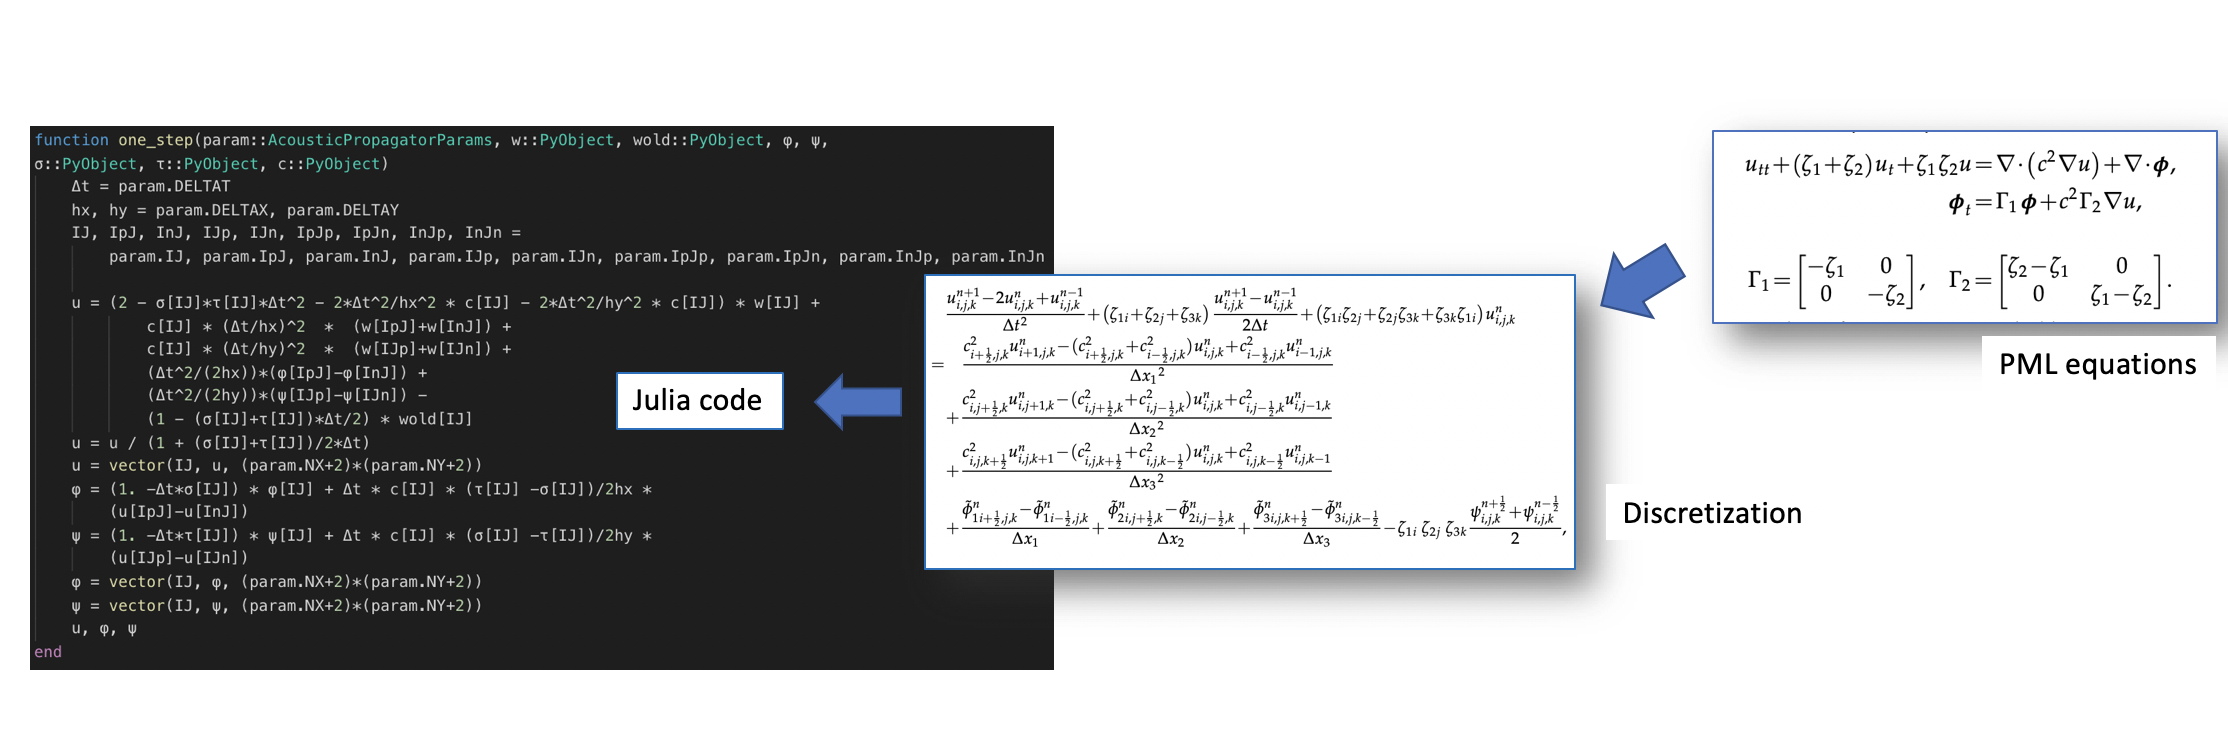
\includegraphics[width=1.0\textwidth]{figures/Julia.png}
\end{figure}
\end{frame}

\begin{frame}
	\frametitle{A General Approach to Inverse Modeling}
	\begin{figure}[hbt]
  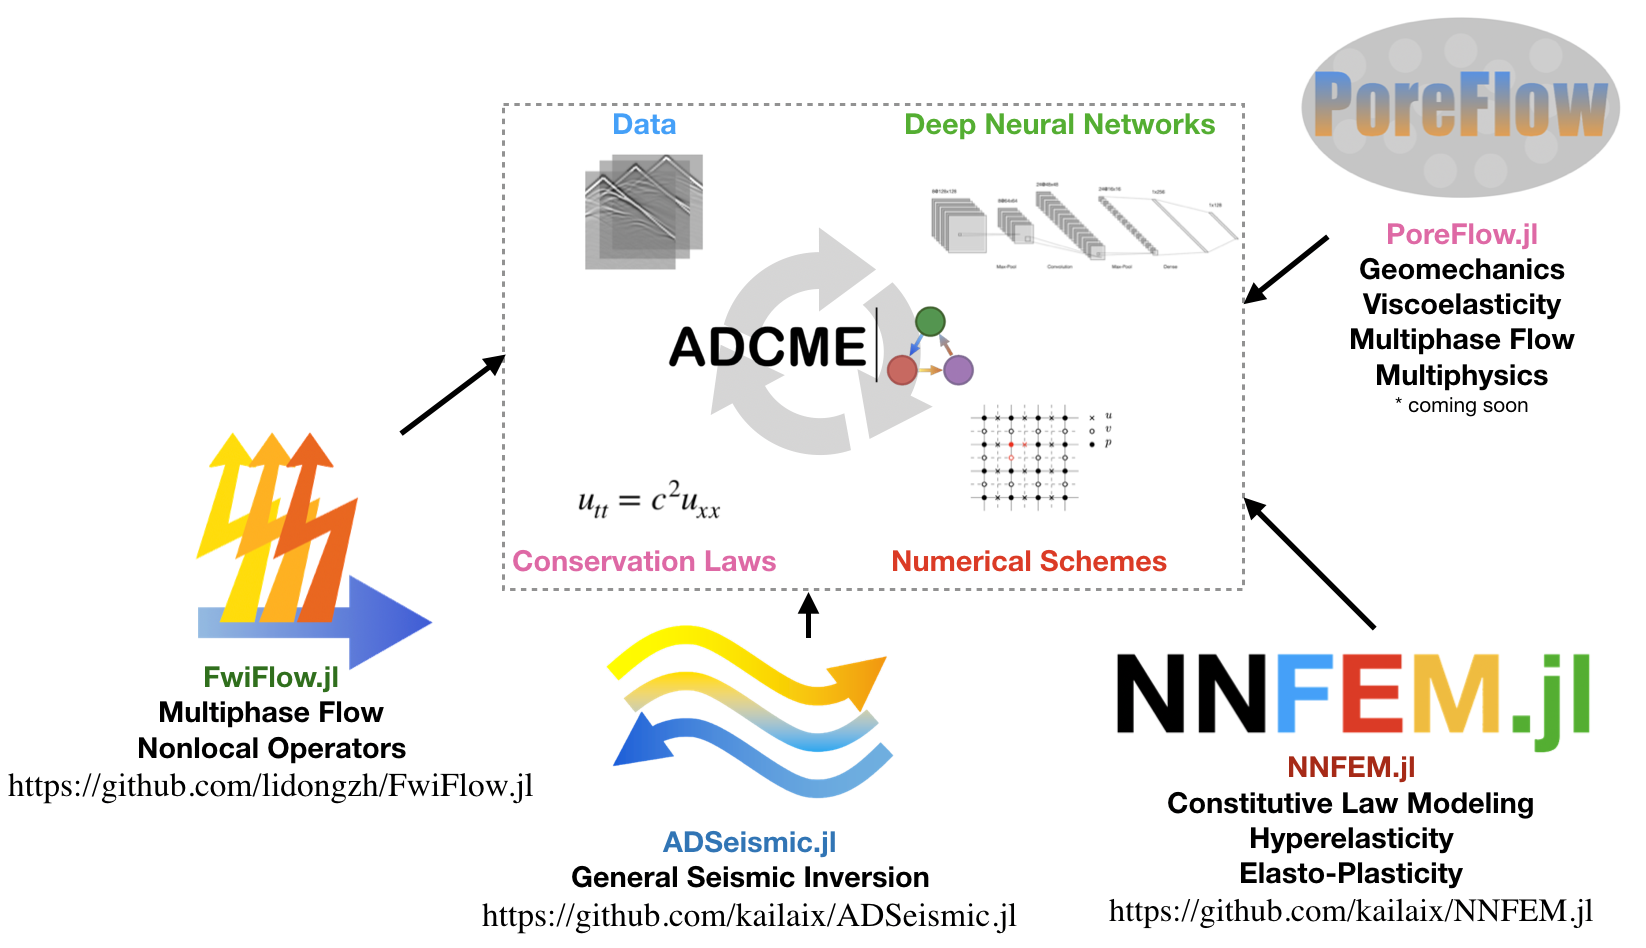
\includegraphics[width=1.0\textwidth]{figures/summary.png}
\end{figure}

\end{frame}

\begin{frame}
	\frametitle{Acknowledgement}
	\begin{itemize}
		\item \texttt{NNFEM.jl}: Joint work with Daniel Z. Huang and Charbel Farhat.
		\item \texttt{FwiFlow.jl}: Joint work with Dongzhuo Li and Jerry M. Harris. 
		\item \texttt{ADSeismic.jl}: Joint work with Weiqiang Zhu and Gregory C. Beroza. 
		\item \texttt{PoreFlow.jl}: Joint work with Alexandre M. Tartakovsky and Jeff Burghardt.
	\end{itemize}
	
\end{frame}


%}
%\usebackgroundtemplate{}
%----------------------------------------------------------------------------------------
%    PRESENTATION SLIDES
%----------------------------------------------------------------------------------------

%------------------------------------------------



\end{document} 